\section{Benchmark Examples}

Since the \MA equation became a benchmark problem for fully nonlinear second order PDEs there are some classical test problems for the two-dimensional case. All test cases are formulate for the domain $\Omega$ to be the unitsquare $[0,1]^2$.

\begin{test} \label{test smooth}
The first classical \MA test is the problem with the data
\[
	u=\exp( \lVert x \rVert_2^2  /2) 
	\text { and } 
	f = (1 + \lVert x \rVert_2^2) \exp( \lVert x \rVert^2).
\]
It has a very smooth solution and is even radial.

\end{test}

\begin{test}\label{test sqrt}
The data
\[
	u = - \sqrt{ 2-  \lVert x \rVert_2^2}
	\text { and } 
	f = 2\left( 2-  \lVert x \rVert_2^2 \right)^{-2}
\]
defines the second example. This test is especially interesting because the convex viscosity solution is only contained in $W^{1,p}(\Omega) $ for $p \in [0,4)$\cite{DG2006a}, i.e. it lacks $H^2$ regularity.
\end{test}

For the next two tests we define $x_0 = \left(\frac 1 2, \frac 1 2  \right)^t$.

\begin{test}\label{test singularity}
The third \MA test is yet more regular. Its solution lies in $C^1$ and it is given by
\[
	u=\frac 1 2 \left( \max 0 {\lVert x - x_0 \rVert_2-0.2 }  \right)^2 
	\text { and } 
	f = \max 0 {1-\frac {0.2} {\lVert x - x_0 \rVert_2} }.
\]
\end{test}


\begin{test}\label{test dirac}
The last test is determined by
\[
	u = \lVert x - x_0 \rVert_2
	\text { and } 
	f = \pi \delta_{x_0}
\]
and its solution $u$ describes a cone with origin $x_0$. This example does not have a viscosity solution, but $u$ is only an Aleksandrov solution of the problem \cite[Section 2.3.]{FO2011}.

Note that $f$ is highly non regular. Motivated by \cite[Section 6.1.]{FO2011} we discretise $f$ by
\begin{align*}
	f_h = \begin{cases}
		\frac \pi {4h^2} & \text{ if} \singleNorm{x_1 - 0.5} \leq h \text{ and } \singleNorm{x_e - 0.5} \leq h \\
		0	& \text{otherwise}
	\end{cases}.
\end{align*}
\end{test}


%\begin{test}\label{test rhsConst}
%A test where the analytical solution is unknown is determined by
%\[
%	u = 0 \text{ on } \partial \Omega
%	\text { and } 
%	f = 1
%\]
%defines the last example.
%\end{test}

\section{Numerical Results of a $C^0$ Penalty Method}\label{sec: numerical results brenner}

%read data for case deg=22 and merge into one file
\newcommand{\readDataN}[2]{
\pgfplotstableread{../../FEniCS/data/#1_l2errornorm} #2

\pgfplotstablecreatecol[copy column from table={../../FEniCS/data/#1_h1errornorm}{h1error}] {h1error} #2

\pgfplotstablecreatecol[copy column from table={../../FEniCS/data/#1_newtonSteps}{steps}] {N} #2
}

%\readDataN{MA1_Brenner_deg2}{\MAOneBrennerTwo}
%\readDataN{MA1_Brenner_deg3}{\MAOneBrennerThree}

%\readDataN{MA3_Brenner_deg2}{\MAThreeBrennerTwo}

%\readDataN{MA4_Brenner_deg2}{\MAFourBrennerTwo}
%\readDataN{MA4_Brenner_deg3}{\MAFourBrennerThree}


\readDataN{MA1_Neilan_GradJump_deg22}{\MAOneJumpdegTwoTwo}
\readDataN{MA1_Neilan_GradJump_deg20}{\MAOneJumpdegTwoZero}

\readDataN{MA1_Neilan_deg33}{\MAOnedegThreeThree}
\readDataN{MA1_Neilan_deg32}{\MAOnedegThreeTwo}

%\readDataN{MA2_Neilan_deg22}{\MATwodegTwoTwo}
%\readDataN{MA2_Neilan_deg33}{\MATwodegThreeThree}

%\readDataN{MA3_Neilan_deg22}{\MAThreedegTwoTwo}
%\readDataN{MA3_Neilan_deg33}{\MAThreedegThreeThree}
\readDataN{MA3_Neilan_GradJump_deg22}{\MAThreeJumpdegTwoTwo}
\readDataN{MA3_Neilan_GradJump_deg33}{\MAThreeJumpdegThreeThree}


%\pgfplotstableread{../../FEniCS/data/MA1_Neilan_deg22_l2errornorm} \MAOnedegTwoTwoL
%\pgfplotstableread{../../FEniCS/data/MA1_NeilanGradJump_deg22_l2errornorm} \MAOneJumpdegTwoTwo
%\pgfplotstableread{../../FEniCS/data/MA1_NeilanGradJump_deg22_h1errornorm}\MAOneJumpdegTwoTwoH

%\pgfplotstablecreatecol[copy column from table={../../FEniCS/data/MA1_NeilanGradJump_deg22_h1errornorm}{h1error}] {h1error} \MAOneJumpdegTwoTwo
%\pgfplotstablecreatecol[copy column from table={../../FEniCS/data/MA1_NeilanGradJump_deg22_newtonsteps}{steps}] {N} \MAOneJumpdegTwoTwo


For reference I implemented the algorithm introduced in Section \ref{sec: Brenner method}.
We implemented their presented method using the finite element tool FEniCS \cite{FEniCS}, the Code is append in Appendix. 
To create our initial guess I did not use a vanishing moment method as Brenner suggested, but the solution of $\triangle u = -\sqrt{2f}$ as introduced in Section \ref{sec: initial guess}. 

The triangulation $\triang$ was obtained by a standard refinement as explained in Section ref{subsec: refinement and base cells}: First the domain was split into four triangles by drawing both diagonals and afterwards each triangle was successively divided into four congruent triangles.
\begin{figure}[H]
	\centering
	\begin{subfigure}{0.45\textwidth}
		\centering
		\edef \n {2}
		\usetikzlibrary{calc}
\begin{tikzpicture}[scale=5]

	\draw (0,0) -- (1,0) -- (1,1) -- (0,1) -- cycle;

	\foreach \x in {0,1,...,\n}
{
	\pgfmathtruncatemacro \y {1-\x/\n}
	\draw (0,\x/\n) -- (1-\x/\n,1);
	\draw (\x/\n,0) -- (1,1-\x/\n);

	\draw (0,\x/\n) -- (\x/\n,0);
	\draw (1,\x/\n) -- (\x/\n,1);

   \draw (\x/\n, \x/\n) -- (1-\x/\n, \x/\n) -- (1-\x/\n, 1-\x/\n) -- (\x/\n, 1- \x/\n) -- cycle;
	\def \y {\x/2/\n}
   \draw (\y, \y) -- (1-\y, \y) -- (1-\y, 1-\y) -- (\y, 1- \y) -- cycle;
}

\end{tikzpicture}
		\caption{Triangulation with $h=\frac 1 2$}
		\label{fig: grid1}
	\end{subfigure}
	\begin{subfigure}{0.45\textwidth}
		\centering
		\edef \n {4}
		\usetikzlibrary{calc}
\begin{tikzpicture}[scale=5]

	\draw (0,0) -- (1,0) -- (1,1) -- (0,1) -- cycle;

	\foreach \x in {0,1,...,\n}
{
	\pgfmathtruncatemacro \y {1-\x/\n}
	\draw (0,\x/\n) -- (1-\x/\n,1);
	\draw (\x/\n,0) -- (1,1-\x/\n);

	\draw (0,\x/\n) -- (\x/\n,0);
	\draw (1,\x/\n) -- (\x/\n,1);

   \draw (\x/\n, \x/\n) -- (1-\x/\n, \x/\n) -- (1-\x/\n, 1-\x/\n) -- (\x/\n, 1- \x/\n) -- cycle;
	\def \y {\x/2/\n}
   \draw (\y, \y) -- (1-\y, \y) -- (1-\y, 1-\y) -- (\y, 1- \y) -- cycle;
}

\end{tikzpicture}
		\caption{Triangulation with $h=\frac 1 4$}
		\label{fig: grid}
	\end{subfigure}	
	\caption{Triangulation with $h=\frac 1 4$}
	\label{fig: grids}
\end{figure}

The arising nonlinear system is solved by PETSc configured with FEniCS default solver choice: That is a Newton based nonlinear solver that uses a line search and the arising linear systems are solved by a $LU$ decomposition.
%SNES Object: 1 MPI processes
%  type: newtonls
%  SNES has not been set up so information may be incomplete
% maximum iterations=10, maximum function evaluations=2000
% tolerances: relative=1e-09, absolute=1e-08, solution=1e-16
%total number of linear solver iterations=0
%total number of function evaluations=0
%SNESLineSearch Object:   1 MPI processes
% type: bt
%  interpolation: cubic
%   alpha=1.000000e-04
%  maxstep=1.000000e+08, minlambda=1.000000e-12
%   tolerances: relative=1.000000e-08, absolute=1.000000e-15, lambda=1.000000e-08
%  maximum iterations=40
%KSP Object:   1 MPI processes
%type: preonly
%maximum iterations=10000, initial guess is zero
% tolerances:  relative=1e-05, absolute=1e-50, divergence=10000
% left preconditioning
% using DEFAULT norm type for convergence test
%PC Object:   1 MPI processes
%  type: lu
%  PC has not been set up so information may be incomplete
%  LU: out-of-place factorization
%   tolerance for zero pivot 2.22045e-14
%   matrix ordering: nd
% linear system matrix = precond matrix:
% Matrix Object:     1 MPI processes
%  type: seqaij
%  rows=112, cols=112
%  total: nonzeros=2744, allocated nonzeros=2744
%  total number of mallocs used during MatSetValues calls =0
%  using I-node routines: found 80 nodes, limit used is 5
Only the absolute tolerance and the number of maximum iteration are changed from the original default values, the absolute tolerance is adjusted to $1e-8$ and the number of maximum iteration restricted to 100. 

The results can be found in figure \ref{fig: Brenner test1} and in table \ref{tab: l2 errors test 1 Brenner} where $h$ denotes the grid width and $N$ denotes the iterations needed to reach the desired tolerance. 

\begin{table}[H]
	\begin{subtable}[b]{0.45\textwidth}
		\centering
		\pgfplotstabletypeset[columns={iterations, l2error, h1error,N},
				    every row 0 column 0/.style={set content=init},
		]\MAOneBrennerTwo
    	\caption{Error for $k=2$}
   \end{subtable}
   ~
	\begin{subtable}[b]{0.45\textwidth}
		\centering
		\pgfplotstabletypeset[columns={iterations, l2error, h1error,N},
				    every row 0 column 0/.style={set content=init},
		]\MAOneBrennerThree
 	\caption{Error for $k=3$}
	\end{subtable}
	\caption{Errors for test case \ref{test smooth}}
	\label{tab: l2 errors test 1 Brenner}
\end{table}

Fitting the data we can calculate the numerical convergence order $2.502$ for $k=2$ and $3.584$ for $k=3$ in the $L^2$ error norm as well as $2.007$ for $k=2$ and $3.028$ in the $H^1$ error norm. Thus, the results in the $H^1$ confirm the almost convergence rate $k$ as predicted by the authors (cf. also Theorem \ref{thm: error estimate brenner}).
Additionally we observe that the method also converges for polynomial degree $k=2$ with optimal rates although the prove of the error estimate do not cover the case $k<3$.

\begin{figure}[H]
\centering
	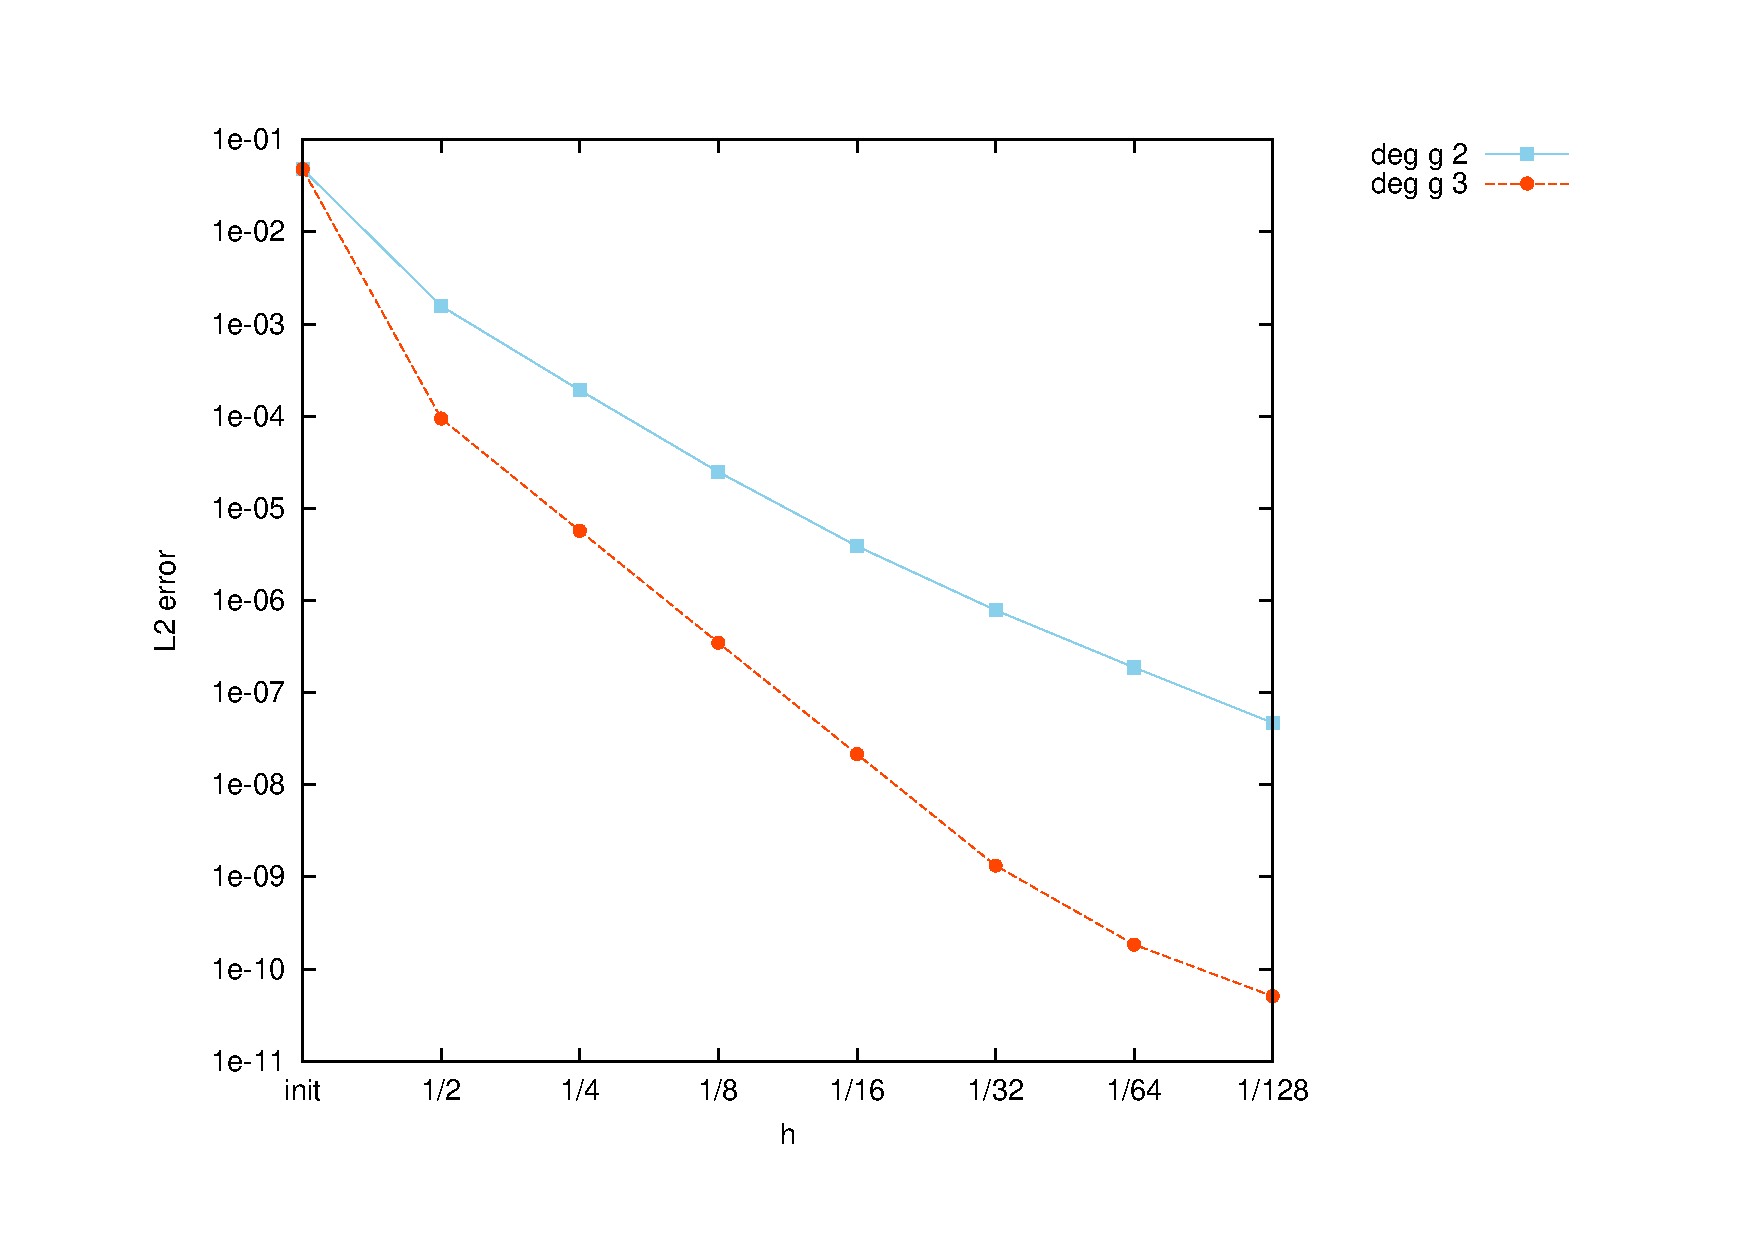
\includegraphics[scale=0.45]{../../FEniCS/diagrams/MA1_Brenner_l2.pdf}
	\caption{$L^2$ errors for test case \ref{test smooth}}
	\label{fig: Brenner test1}
\end{figure}
\begin{figure}[H]
	\centering
	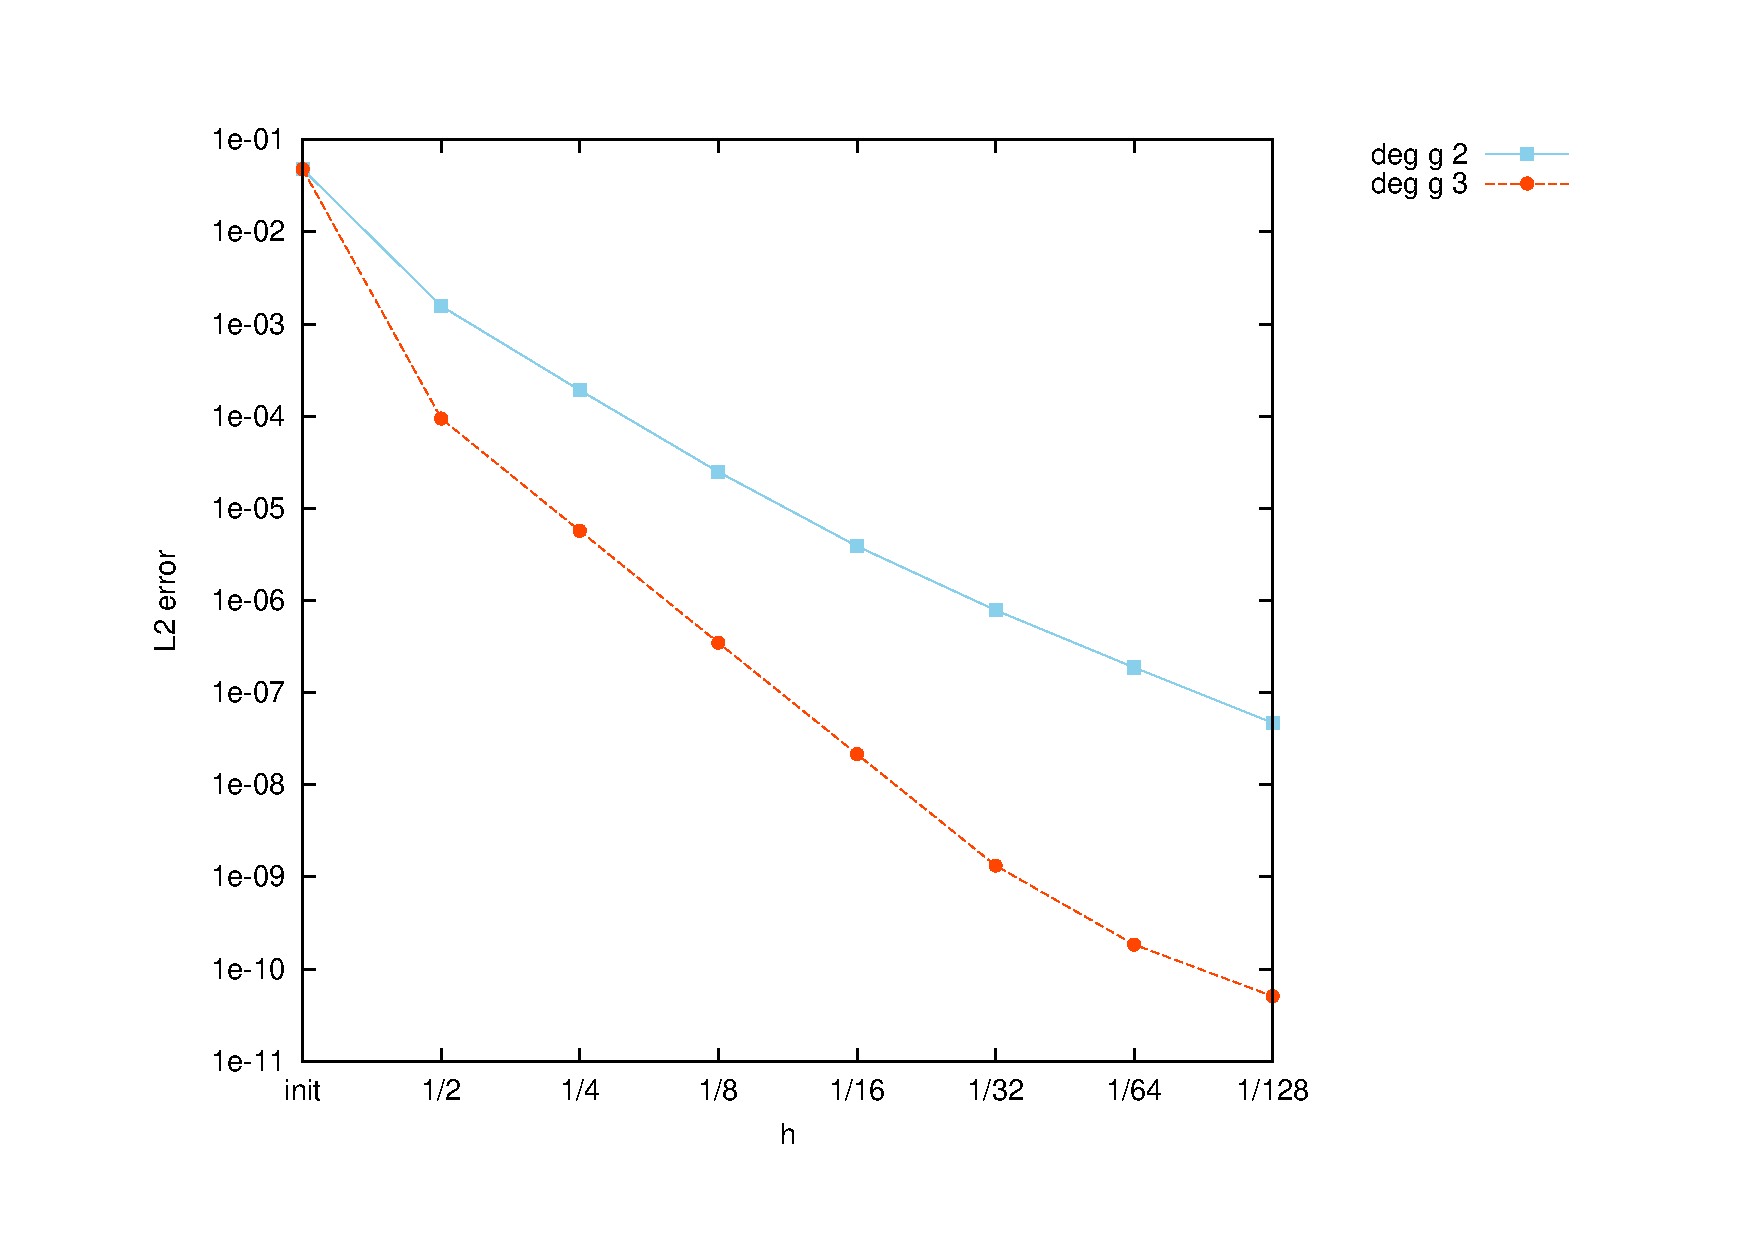
\includegraphics[scale=0.45]{../../FEniCS/diagrams/MA1_Brenner_l2.pdf}
	\caption{$H^1$ errors for test case \ref{test smooth}}
	\label{fig: Brenner test1 h1}
\end{figure}

For the second test case the Newton did not converge, not even on the coarsest grid. Also in the third test case our Newton solver had problems. You can see results of the runs for $h=1/2, \dots, 1/16$ in table \ref{tab: l2 errors test 3 Brenner}, for finer grid the solver did not converge. Attempts to solve this example with FEniCS' built in damped Newton method with different relaxation parameters did also not succeed on any grid finer than $1/16$.
\begin{table}[h]
		\centering
		\pgfplotstabletypeset[columns={iterations, l2error, h1error,N},
				    every row 0 column 0/.style={set content=init},
		]\MAThreeBrennerTwo
    	\caption{Error for $k=2$}
	\caption{Errors for test case \ref{test singularity}}
	\label{tab: l2 errors test 3 Brenner}
\end{table}

The fourth example does not have not a classical solution. As in the previous cases the method does not converge. The corresponding results are shown in table \ref{tab: l2 errors test 4 Brenner}.

\begin{table}[H]
	\begin{subtable}[b]{0.45\textwidth}
		\centering
		\pgfplotstabletypeset[columns={iterations, l2error, h1error,N},
				    every row 0 column 0/.style={set content=init},
				    columns/l2error/.style={ /pgf/number format/sci precision=6}     % print 14 digits
		]\MAFourBrennerTwo
    	\caption{Error for $k=2$}
   \end{subtable}
   ~
	\begin{subtable}[b]{0.45\textwidth}
		\centering
		\pgfplotstabletypeset[columns={iterations, l2error, h1error,N},
				    every row 0 column 0/.style={set content=init},
				    columns/l2error/.style={ /pgf/number format/sci precision=6}     % print 14 digits
		]\MAFourBrennerThree
 	\caption{Error for $k=3$}
	\end{subtable}
	\caption{Errors for test case \ref{test dirac}}
	\label{tab: l2 errors test 4 Brenner}
\end{table}

%For the last test case with constant right-hand side and zero Dirichlet boundary data Newton's method only converged on the coarsest grid such that we cannot make any statement on this test.

We see that this method behaves well for smooth solutions for which it was designed. The results show that it is inappropriate for problems with non smooth-solution or viscosity solutions.

\section{Numerical Results of a Finite Element Method based on a Disrete Hessian}

Also the Neilan's algorithm \cite{Neilan2014} introduced in Section \ref{sec: FEM discrete Hessian} was implemented.
Additional to the numerical results on convergence which Neilan already presented it is interesting to explore what happens if we vary the polynomial degree for the Hessian ansatz space. 

The implementation was also done with the Finite Element Tool FEniCS \cite{FEniCS}, the corresponding source code can be found in the appendix \ref{app: Code Neilan}. \\
The uniform triangulation $\triang$ is the same as in the scenarios for the $C^0$ penalty method (cf. Section \ref{sec: numerical results brenner})
Different to the initial guess suggested in \cite{Neilan2014} I used the solution of $\triangle u = -\sqrt{2f}$ as introduced in Section \ref{sec: initial guess}. All results presented base on discontinuous ansatz spaces, namely piecewise polynomial spaces as introduced in \ref{def: piecewise polySpace}.

We denote the degree of the trial space $V_h=\mathcal P_h^k$ by $k$ and the degree chosen for the Hessian ansatz space $\Sigma_h = [\mathcal{P}_h^{k_{DH}}]^{d \times d}$ by $k_{DH}$. The solver for nonlinear system of equations given by \eqref{eq: neilan eq1} and \eqref{eq: discrete hessian} or \eqref{eq: neilan eq1 + jump} and \eqref{eq: discrete hessian} is configured with the same paramters as in the previous section if not stated otherwise. 


Figure \ref{fig: l2 errors test 1} shows the $L^2$ error of all performances of the first test case that have converged, the polynomial degrees $k$ were taken to be $1,\dots,3$ and $k_{DH}$ equal to all variants $0, \dots, k$. In Figure \ref{fig: h1 errors test 1} the corresponding $H^1$ errors are plotted.

Due to the large number of degree of freedoms the requested memory for the cases $k=2,3$ and $k_{DH}=2,3$ on the finest grid, for $k=3$ and $k_{DH}=3$ all meshes with $h\geq 1/64$ is too much. Replacing the linear solver by different iterative solvers\footnote{GMRES with an algebraic multigrid preconditioner, GMRES with an incomplete $LU$ factorisation, GMRES with Jacobi preconditioning, bicgstab with preconditioning} yielded to divergence of either the Newton or the linear solver.

\begin{figure}[H]
\centering
	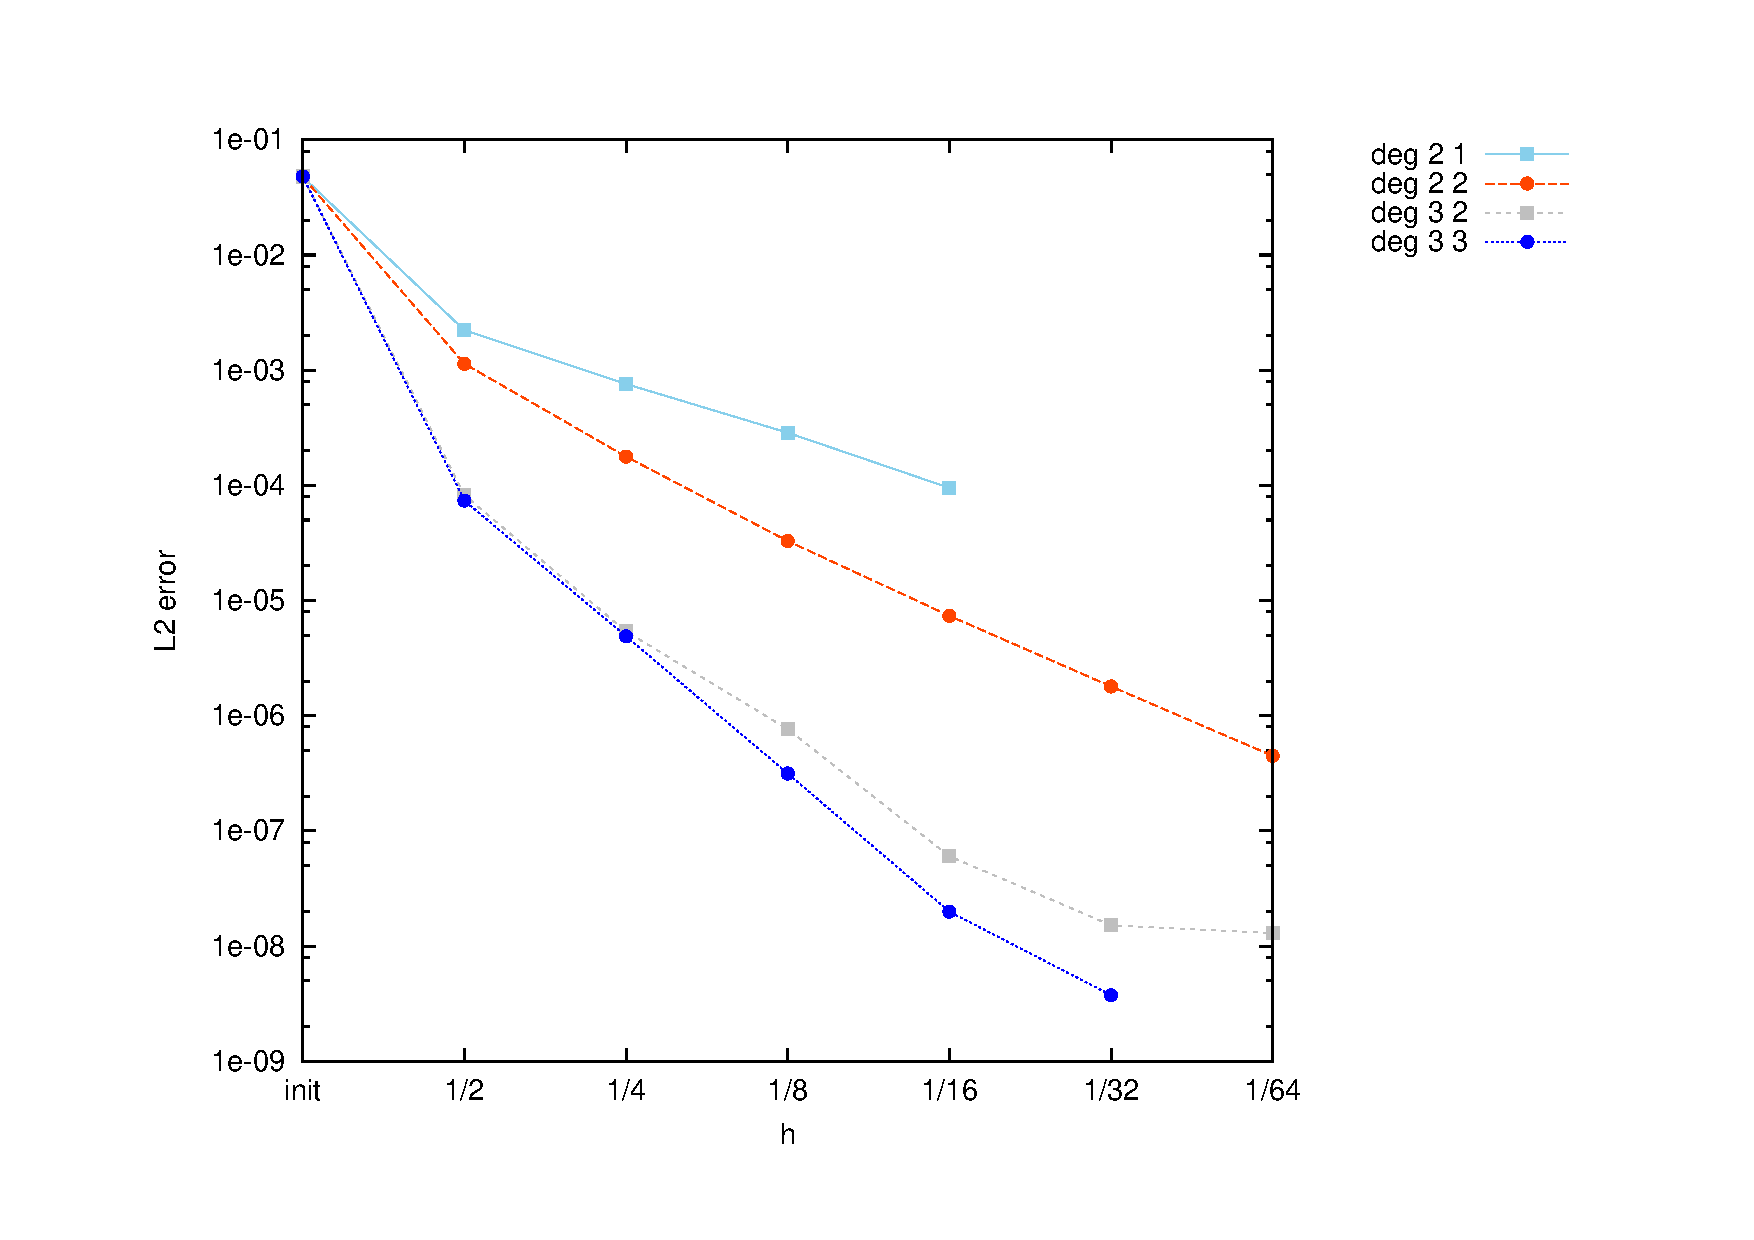
\includegraphics[scale =0.45]{plots/MA1_Neilan_l2.pdf}
	\caption{$L^2$ errors for test case \ref{test smooth}}
	\label{fig: l2 errors test 1}
\end{figure}
The results for the runs with $k=3$ are shown more detailed in Table \ref{tab: l2 errors test 1 deg 2}, in both tables the column $N$ refers to the number of iterations the Newton solver needed to reach the desired tolerance. 
\begin{table}[H]
	\begin{subtable}[b]{0.45\textwidth}
		\centering
		\pgfplotstabletypeset[columns={iterations, l2error, h1error,N},
		every row 0 column 0/.style={set content=init},
		every row 6 column 1/.style={set content=-},
		every row 6 column 2/.style={set content=-},
		every row 6 column 3/.style={set content=-},
		]\MAOnedegThreeThree
		\caption{Error for $k=3, k_{DH}=3$}
	\end{subtable}
	~
	\begin{subtable}[b]{0.45\textwidth}
		\centering
		\pgfplotstabletypeset[columns={iterations, l2error, h1error,N},
		every row 0 column 0/.style={set content=init},
		]\MAOnedegThreeTwo
		\caption{Error for $k=3, k_{DH}=2$}
	\end{subtable}
	\caption{Errors for test case \ref{test smooth}}
	\label{tab: l2 errors test 1 deg 2}
\end{table}


\begin{figure}[H]
\centering
	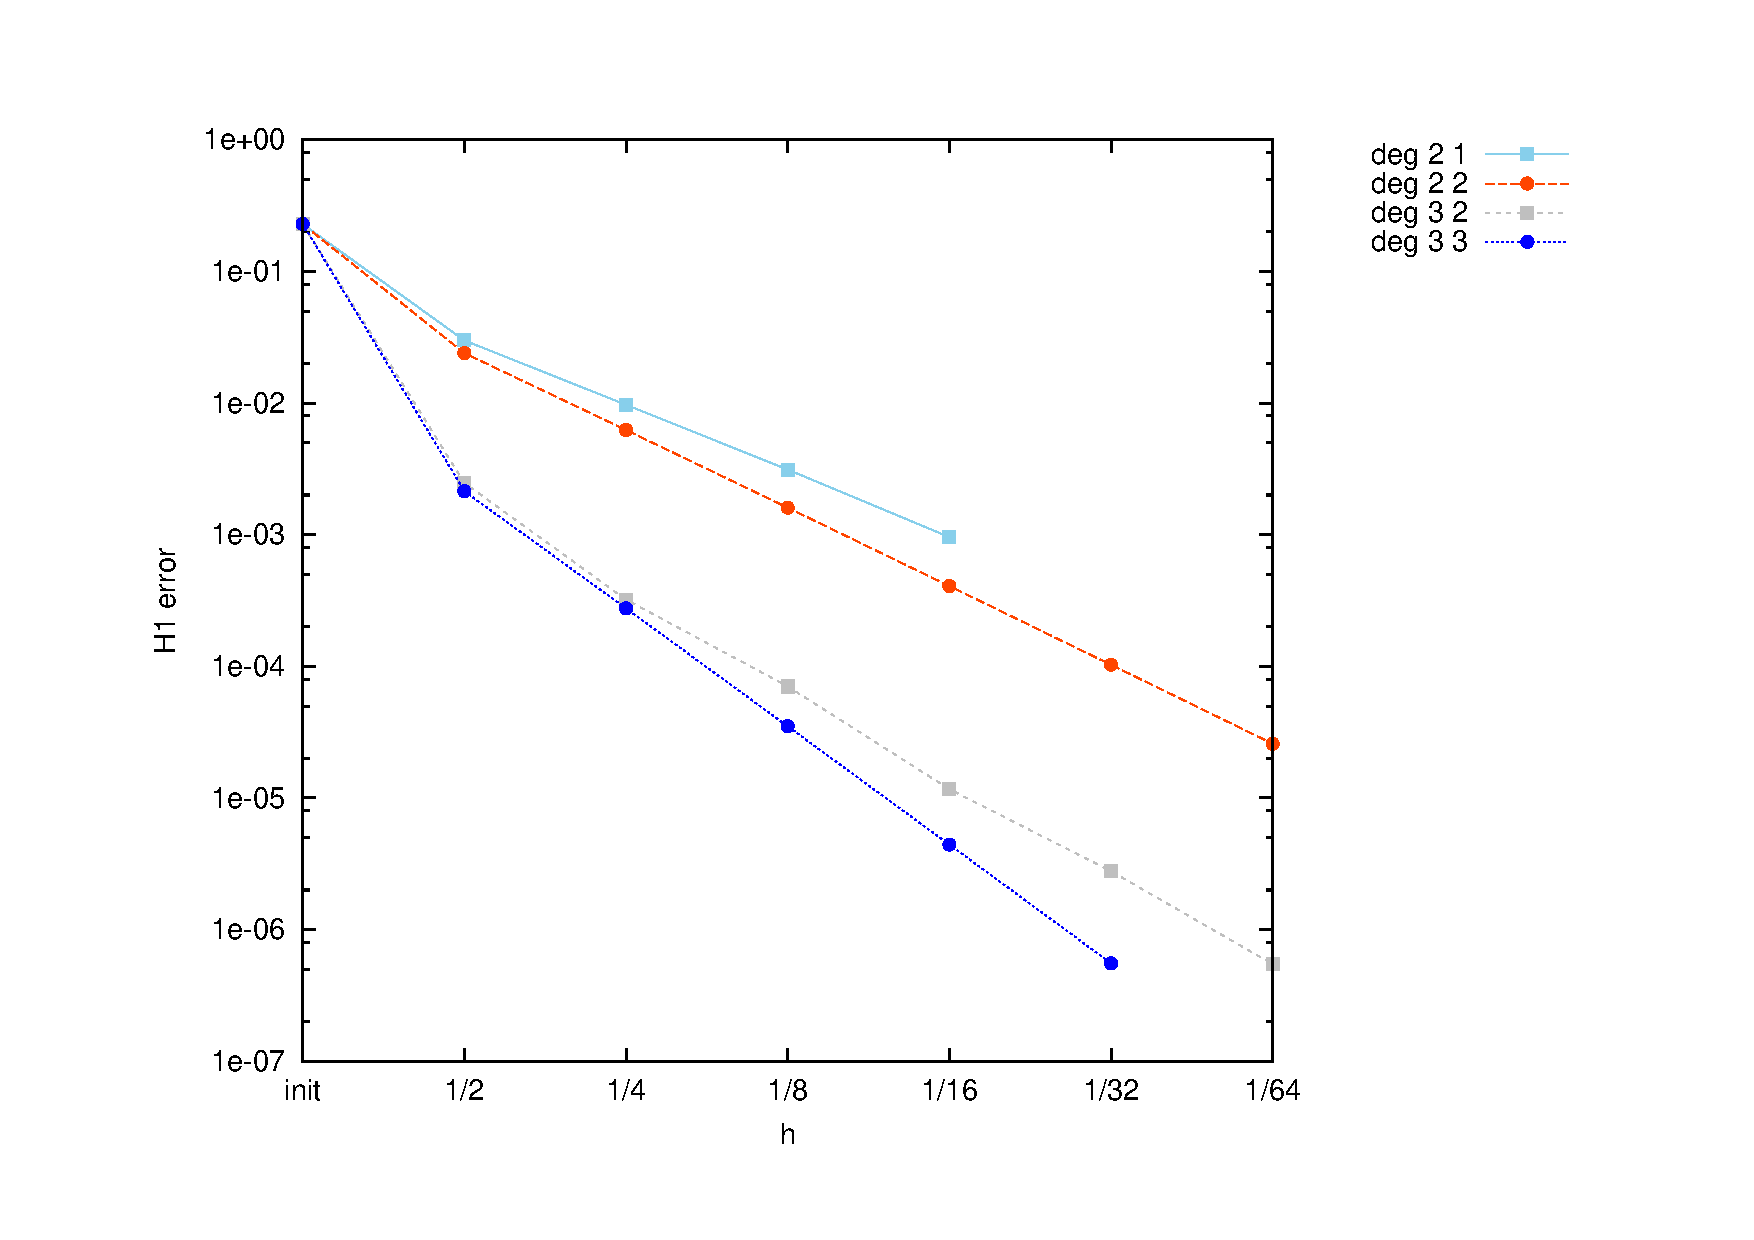
\includegraphics[scale =0.45]{plots/MA1_Neilan_h1.pdf}
	\caption{$H^1$ errors for test case \ref{test smooth}}
	\label{fig: h1 errors test 1}
\end{figure}

As also experienced by Neilan the method does not work for the polynomial degree $k=1$. Similarly, in runs with a low polynomial degree $k_{DH}$ Newton's method did not converge.
Considering this results in the smooth test scenario we observe that the error almost do not alter for different polynomial degrees $k_{DH}$ if both converge. Albeit for fine grids the methods with less difference between the two degrees seem to perform better. The calculated numerical orders as shown in table \ref{tab: order} supports this first intuition.

\begin{table}[H]
\begin{subtable}[b]{0.45\textwidth}
\centering
	\pgfplotstabletypeset
	{
		k $k_{DH}$ {numerical order}
		2 1  1.50338
		2 2  2.24427
		3 2 2.63597
		3 3 3.64758
	}
	\caption{numerical order in $L^2$ norm}
\end{subtable}
\begin{subtable}[b]{0.45\textwidth}
	\pgfplotstabletypeset
	{
		k $k_{DH}$ {numerical order}
		2 1  1.65382 
		2 2  1.973
		3 2 2.39616
		3 3 2.97876
	}
	\caption{numerical order in $H1$ norm}
	\end{subtable}
\caption{numerical order in test \ref{test smooth}}
\label{tab: order}
\end{table}

This test scenario was also performed with the additional normal jump penalty term as proposed by Neilan and stated in \eqref{eq: neilan eq1 + jump} weighted with $\eta$. Fortunately, the method also converges if the linear solver was set to GMRES preconditioned by an incomplete $LU$ factorisation. Thus, the nonlinear solver was adjusted. The results are shown in Figure \ref{fig: l2 errors test 1 jump} and the Tables \ref{tab: l2 errors test 1 deg 2 jump} and \ref{tab: l2 errors test 1 deg 3 jump}. 

\begin{figure}[h!]
\centering
	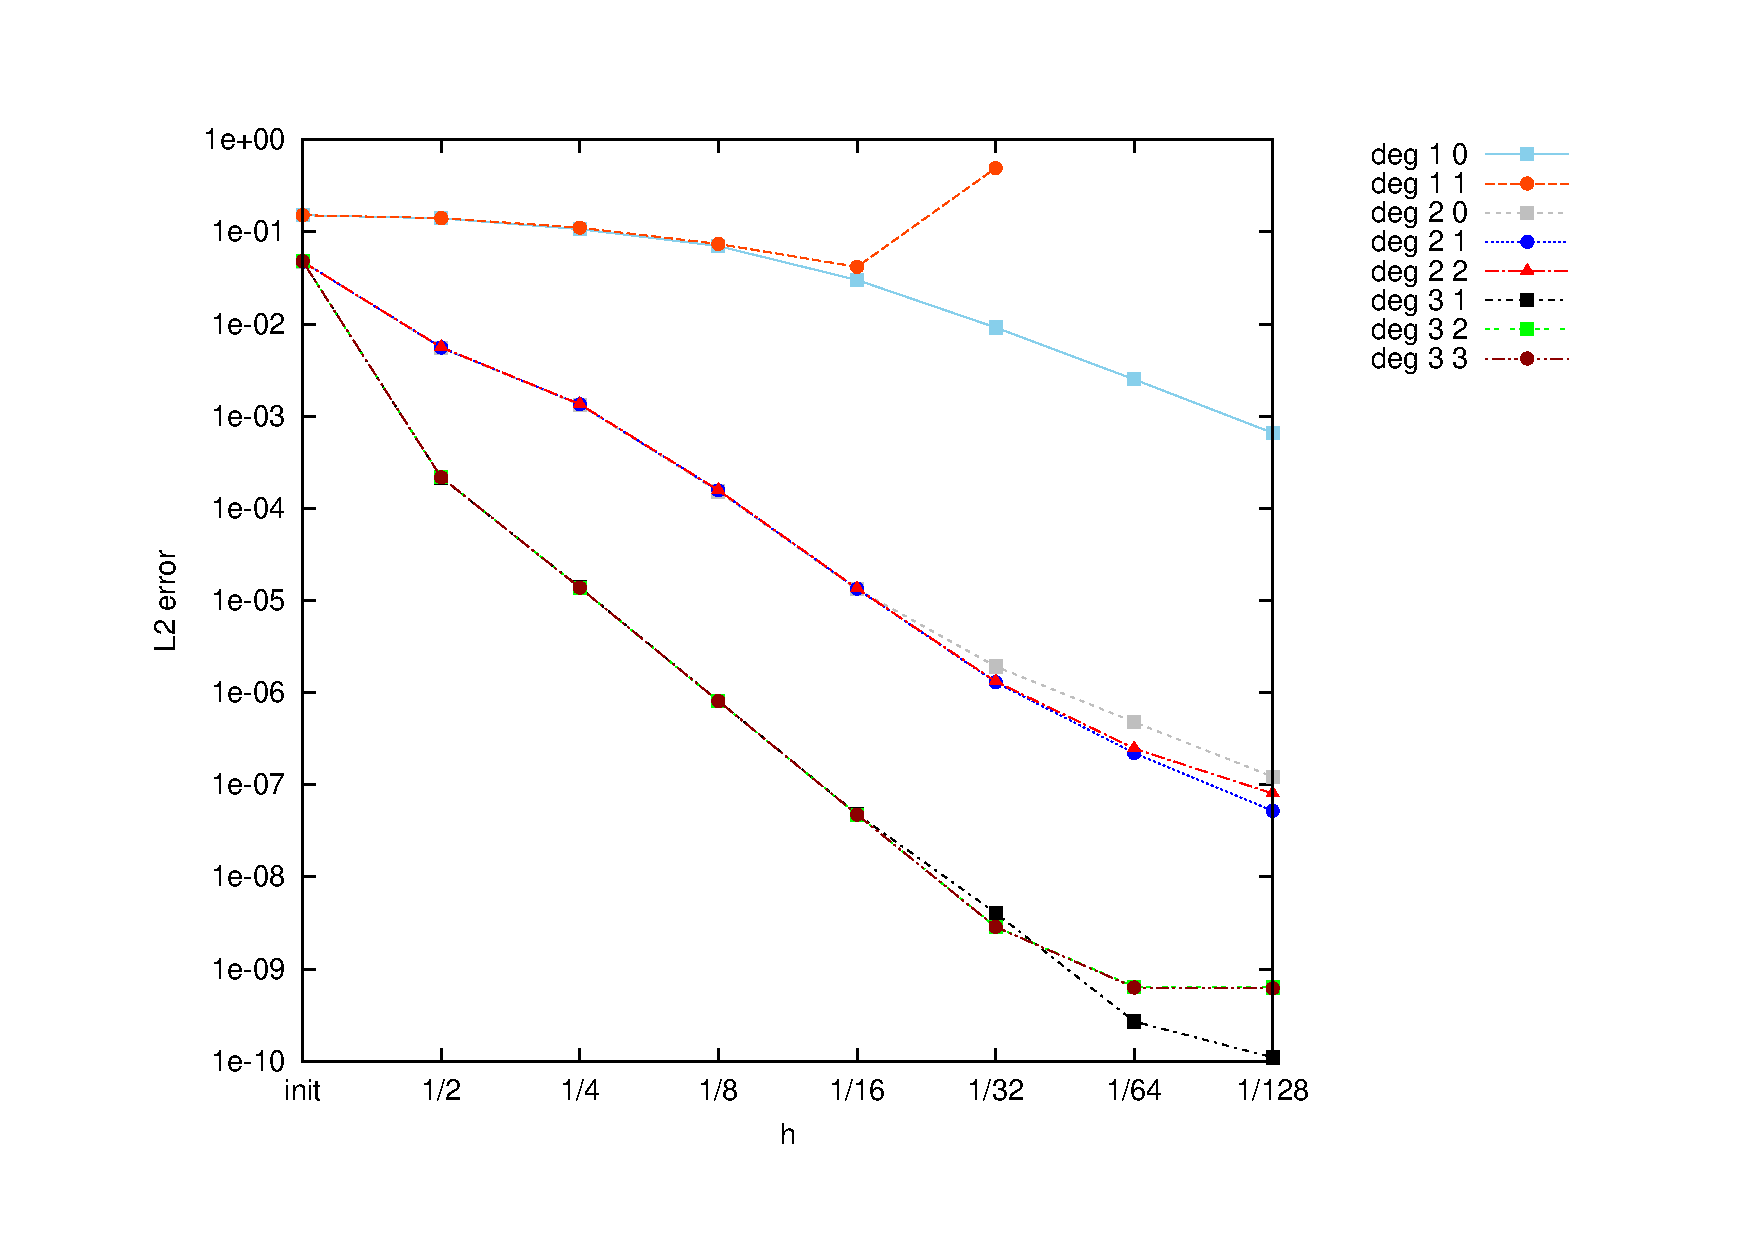
\includegraphics[scale=0.45]{plots/MA1_Neilan_GradJump_l2.pdf}
	\caption{$L^2$ errors for test case \ref{test smooth} and additional gradient jump penalty}
	\label{fig: l2 errors test 1 jump}
\end{figure}
\begin{table}[H]
	\begin{subtable}[b]{0.4\textwidth}
		\centering
		\pgfplotstabletypeset[
		columns={iterations, l2error, h1error,N},
		every row 0 column 0/.style={set content=init},
		]\MAOneJumpdegTwoTwo
		\caption{Error for $k=2, k_{DH}=2$}
	\end{subtable}
	~
	\begin{subtable}[b]{0.4\textwidth}
		\centering
		\pgfplotstabletypeset[columns={iterations, l2error, h1error,N},
		every row 0 column 0/.style={set content=init},
		]\MAOneJumpdegTwoZero
		\caption{Error for $k=2, k_{DH}=0$}
	\end{subtable}
	\caption{Errors for test case \ref{test smooth} with additional jump penalty}
	\label{tab: l2 errors test 1 deg 2 jump}
\end{table}
\begin{table}[h]
	\begin{subtable}[b]{0.45\textwidth}
		\centering
		\pgfplotstabletypeset[
		columns={iterations, l2error, h1error,N},
		every row 0 column 0/.style={set content=init},
		]\MAOneJumpdegThreeThree
		\caption{Error for $k=3, k_{DH}=3$}
	\end{subtable}
	~
	\begin{subtable}[b]{0.45\textwidth}
		\centering
		\pgfplotstabletypeset[columns={iterations, l2error, h1error,N},
		every row 0 column 0/.style={set content=init},
		]\MAOneJumpdegThreeTwo
		\caption{Error for $k=3, k_{DH}=2$}
	\end{subtable}
	\caption{Errors for test case \ref{test smooth} with additional jump penalty}
	\label{tab: l2 errors test 1 deg 3 jump}
\end{table}

\begin{figure}[H]
\centering
	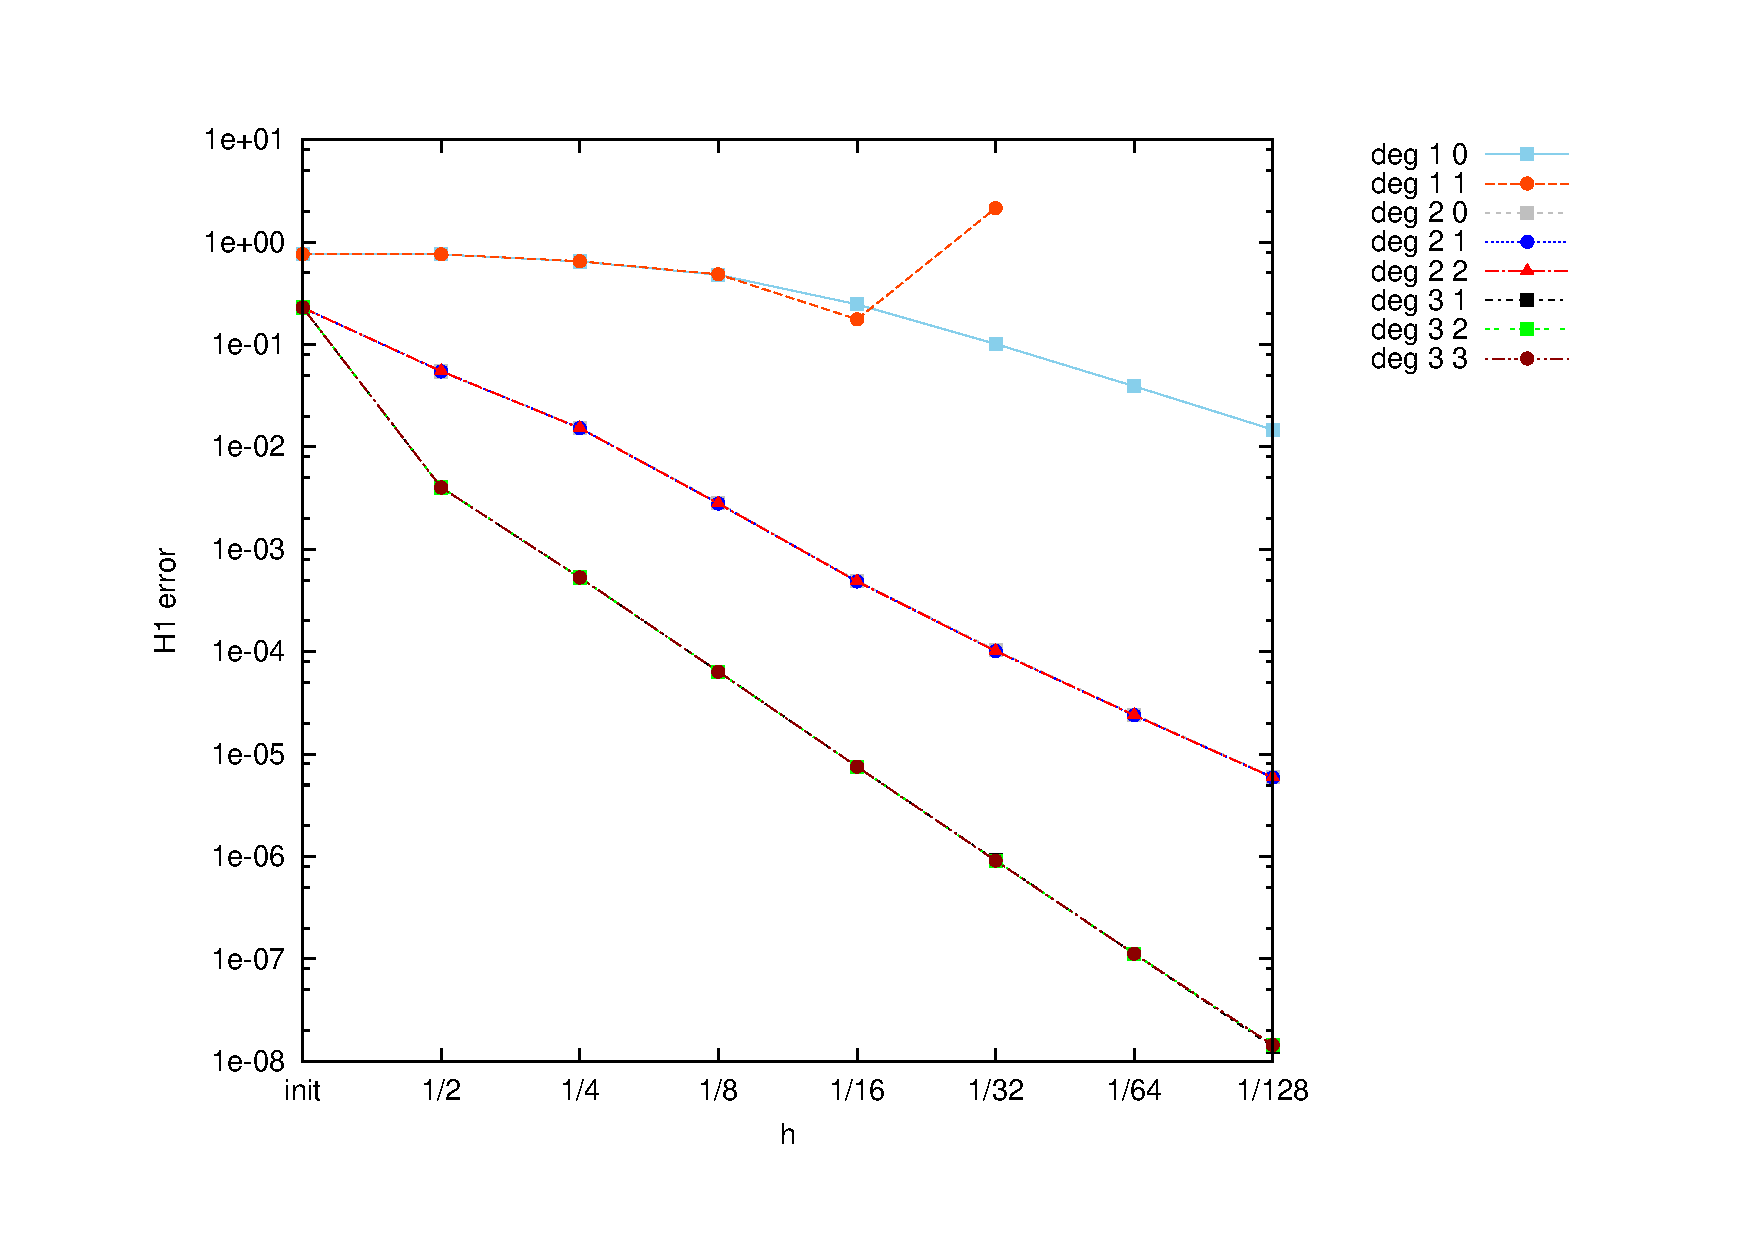
\includegraphics[scale =0.45]{plots/MA1_Neilan_GradJump_h1.pdf}
	\caption{$H^1$ errors for test case \ref{test smooth} and additional gradient jump penalty}
	\label{fig: h1 errors test 1 jump}
\end{figure}

As claimed by Neilan the additional penalisation leads to a convergend method even for low polynomial degrees, even in the cases where only $k_{DH}$ was taken to be small. The only exception is the case $k=1, k_{DH}=1$, for some reason here the method fails. Neilan does not provide any results on this choice of polynomial degrees, he only provides results for $k=1, k_{DH}=0$, $k=2, k_{DH}=2$ and $k=3, k_{DH}=3$. 

Note that the penalised method also for higher degrees performs better than the original ones. This is especially true if $k_{DH}$ was chosen lower than $k$. The numerical orders given in \ref{tab: order jump} confirm this impression and we observe again that the $L^2$ error decreases with order $k+1$ and the $H^1$ error with order $k$. 

Again the calculated error norms indicate that variation of $k_{DH}$ results only in a slight loss of accuracy. For the cases $k=$ and $k_{DH} = 2,3$ the errors and hence, in particular the order, are almost equal. 


\begin{table}[H]
\centering
\begin{subtable}[b]{0.45\textwidth}
	\pgfplotstabletypeset
	{
		k $k_{DH}$ {numerical order}
		1 0 1.32061
		2 0 2.69871
		2 1 2.93488
		2 2 3.0406
		3 1 3.63116
		3 2 4.01895
		3 3 4.0588
	}
	\caption{numerical order in $L2$ norm}
	\end{subtable}
	\begin{subtable}[b]{0.45\textwidth}
	\pgfplotstabletypeset
	{
		k $k_{DH}$ {numerical order}
		1 0 0.978853
		2 0 2.24561
		2 1 2.24836
		2 2 2.28606
		3 1 3.03434
		3 2 3.0359
		3 3  3.0343
	}
	\caption{numerical order in $H1$ norm}
	\end{subtable}
	\caption{numerical order with jump penalty in test \ref{test smooth}}
\label{tab: order jump}
\end{table}


The second test was carried out with the same configuration. Again the size of the system matrices exceeded memory and therefore there are not data points for polynomial degrees $k=2,3$ on fine grids. Table \ref{tab: l2 errors test 2} show the decreasing error norms, it shows only two degree pairs for other degree pairs behaved similarly as we can already see in figure \ref{fig: l2 errors test 2} and \ref{fig: h1 errors test 2}.
\begin{figure}[h]
\centering
	
\includegraphics[scale =0.4]{../../FEniCS/diagrams/MA2_Neilan_l2.pdf}
	\caption{$L^2$ errors for test case \ref{test sqrt} }
	\label{fig: l2 errors test 2}
\end{figure}
\begin{figure}[h]
	\centering
	
\includegraphics[scale =0.4]{../../FEniCS/diagrams/MA2_Neilan_h1.pdf}
	\caption{$H^1$ errors for test case \ref{test sqrt} }
	\label{fig: h1 errors test 2}
\end{figure}
\begin{table}[H]
	\begin{subtable}[b]{0.45\textwidth}
		\centering
		\pgfplotstabletypeset[
		columns={iterations, l2error, h1error,N},
		    every row 0 column 0/.style={set content=init},
		]{\MATwodegTwoTwo}
    	\caption{Error for $k=2, k_{DH}=2$}
   \end{subtable}
   ~
	\begin{subtable}[b]{0.45\textwidth}
		\centering
		\pgfplotstabletypeset[columns={iterations, l2error, h1error,N},
		    every row 0 column 0/.style={set content=init},
		]{\MATwodegThreeThree}
	\caption{Error for $k=3, k_{DH}=3$}
	\end{subtable}
	\caption{Errors for test case \ref{test sqrt}}
	\label{tab: l2 errors test 2}
\end{table}

\begin{table}[H]
\centering
\begin{subtable}[b]{0.45\textwidth}
	\pgfplotstabletypeset
	{
		k $k_{DH}$ {numerical order}
		2 1 1.55213
		2 2 1.63088 
		3 2 1.64644
		3 3 1.64841
	}
	\caption{numerical order in $L2$ norm}
	\end{subtable}
	\begin{subtable}[b]{0.45\textwidth}
	\pgfplotstabletypeset
	{
		k $k_{DH}$ {numerical order}
		2 1 0.465187
		2 2 0.473759
		3 2 0.475829
		3 3  0.495565
	}
	\caption{numerical order in $H1$ norm}
	\end{subtable}
	\caption{numerical order with jump penalty in test \ref{test smooth}}
\label{tab: order jump test 2}
\end{table}

Switching the penalisation of gradient jumps on the method performs again well, its results are shown in figure \ref{fig: l2 errors test 2 jump} and the tables . 
\begin{figure}[H]
\centering
\begin{subfigure}{\textwidth}
\centering
	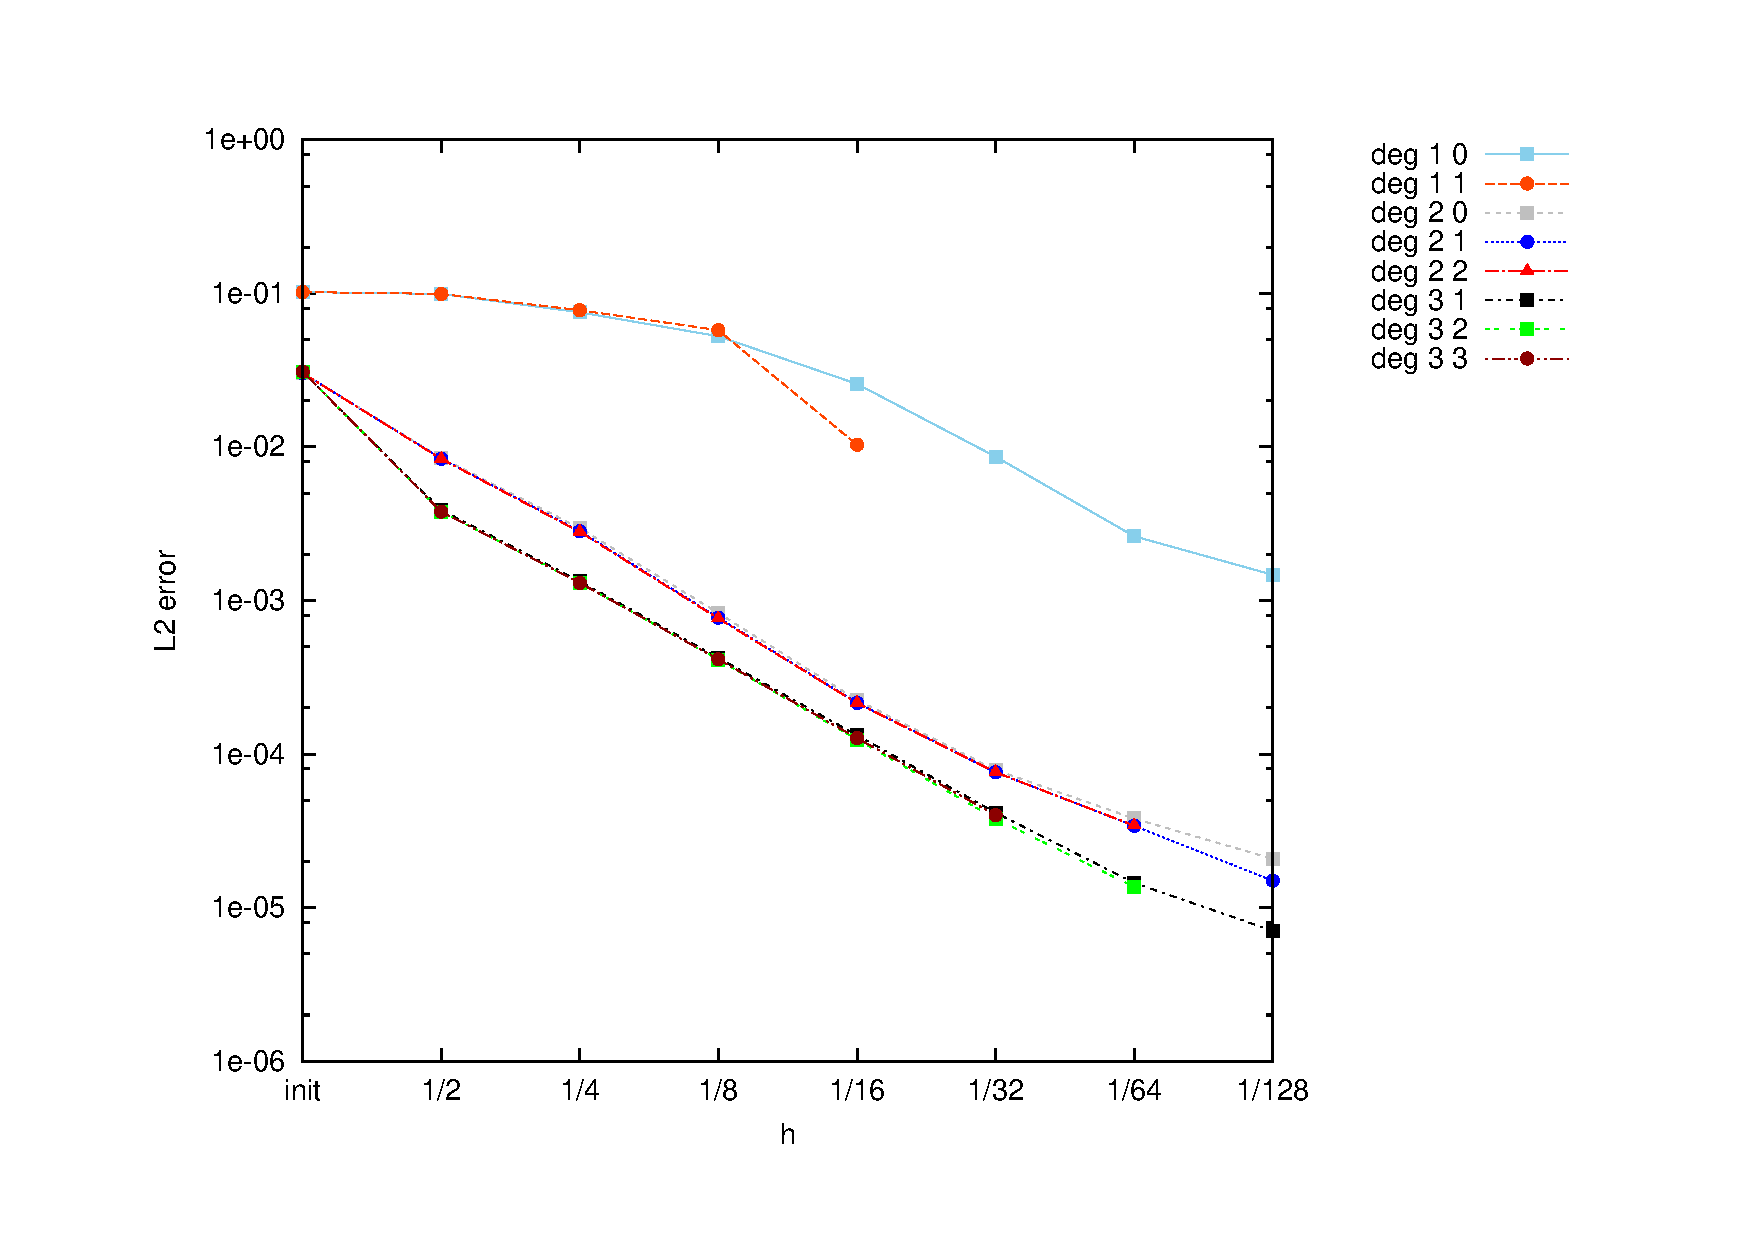
\includegraphics[scale =0.4]{../../FEniCS/diagrams/MA2_Neilan_GradJump_l2.pdf}
\end{subfigure}

\begin{subfigure}{\textwidth}
\centering
	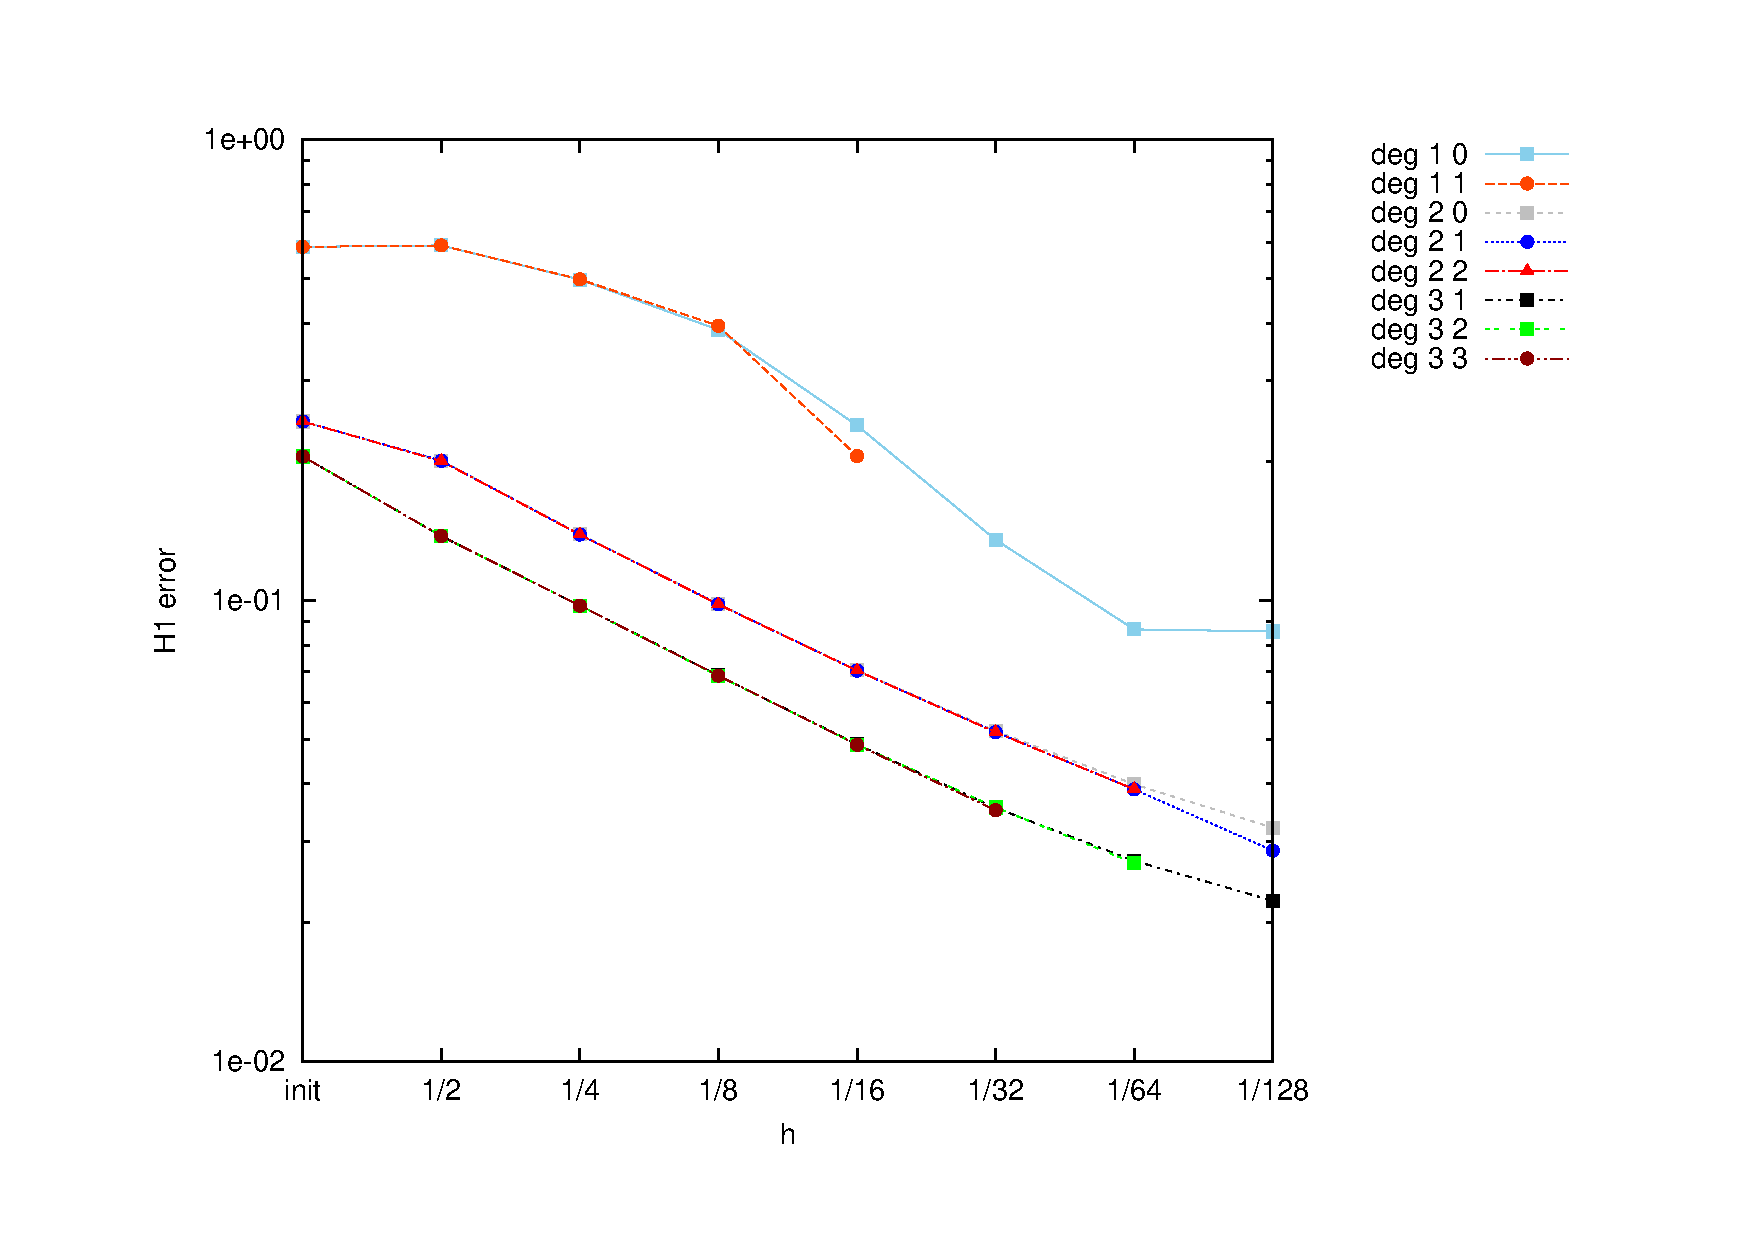
\includegraphics[scale =0.4]{../../FEniCS/diagrams/MA2_Neilan_GradJump_h1.pdf}
\end{subfigure}
	\caption{$L^2$ and $H^1$ errors for test case \ref{test sqrt} and additional gradient jump penalty}
	\label{fig: l2 errors test 2 jump}
\end{figure}
\begin{table}[H]
	\begin{subtable}[b]{0.45\textwidth}
		\centering
		\pgfplotstabletypeset[
		columns={iterations, l2error, h1error,N},
		every row 0 column 0/.style={set content=init},
		]{\MATwoJumpdegTwoTwo}
		\caption{Error for $k=2, k_{DH}=2$}
	\end{subtable}
	~
	\begin{subtable}[b]{0.45\textwidth}
		\centering
		\pgfplotstabletypeset[columns={iterations, l2error, h1error,N},
		every row 0 column 0/.style={set content=init},
		]{\MATwoJumpdegThreeThree}
		\caption{Error for $k=3, k_{DH}=3$}
	\end{subtable}
	\caption{Errors for test case \ref{test sqrt} with additional }
	\label{tab: l2 errors test 2 jump}
\end{table}

As we can see the results do not alter between the method with or without additional penalty on the gradient. Therefore also the numerical orders are almost identical.  
%\begin{table}[H]
%\centering
%\begin{subtable}[b]{0.45\textwidth}
%	\pgfplotstabletypeset
%	{
%		k $k_{DH}$ {numerical order}
%		1 0 1.03719 
%		2 1 1.55213
%		2 2 
%		3 2 
%		3 3 
%	}
%	\caption{numerical order in $L2$ norm}
%	\end{subtable}
%	\begin{subtable}[b]{0.45\textwidth}
%	\pgfplotstabletypeset
%	{
%		k $k_{DH}$ {numerical order}
%		2 1 
%		2 2 
%		3 2 
%		3 3  
%	}
%	\caption{numerical order in $H1$ norm}
%	\end{subtable}
%	\caption{numerical order with jump penalty in test \ref{test smooth}}
%\label{tab: order jump test 2}
%\end{table}


Similar are results for Test \ref{test singularity}, also a problem without a classical solution. Without additional gradient penalty the method does not work well as could be seen in Table \ref{tab: l2 errors test 3} where all converged iteration steps for polynomial degree $k=2, k_{DH}=2$ are shown.
\begin{table}[H]
%	\begin{subtable}[b]{0.45\textwidth}
		\centering
		\pgfplotstabletypeset[
		columns={iterations, l2error, h1error,N},
		    every row 0 column 0/.style={set content=init},
		]{\MAThreedegTwoTwo}
%   \end{subtable}
%   ~
%	\begin{subtable}[b]{0.45\textwidth}
%		\centering
%%		\pgfplotstabletypeset[columns={iterations, l2error, h1error,N},
%%		    every row 0 column 0/.style={set content=init},
%%		]{\MAThreedegThreeThree}
%	\caption{Error for $k=3, k_{DH}=3$}
%	\end{subtable}
	\caption{Errors for Test \ref{test singularity} for $k=2, k_{DH}=2$}
	\label{tab: l2 errors test 3}
\end{table}

The results of the corresponding method with additional jump penalisation can be found in Figure \ref{fig: l2 errors test 3 jump} and Figure \ref{fig: h1 errors test 3 jump}, as well as in Table \ref{tab: l2 errors test 3 jump}. 

As in Test \ref{test smooth} the pair $k=1$ and $k_{DH}=1$ induces a unstable method. We further observe that the method with $k=2$ performs well on coarse grids, whereas for $k=3$ Newton's method does not converge on the coarsest grid. 

The numerical orders given in Table \ref{tab: order jump 3} show the error decreases faster for quadratic polynomials during the first refinements. Yet, for grids with $h \geq \frac 1 {32}$ only the pairing $k=1$ and $k_{DH} =0$ yields to convergence.

\begin{figure}[H]
	\centering
	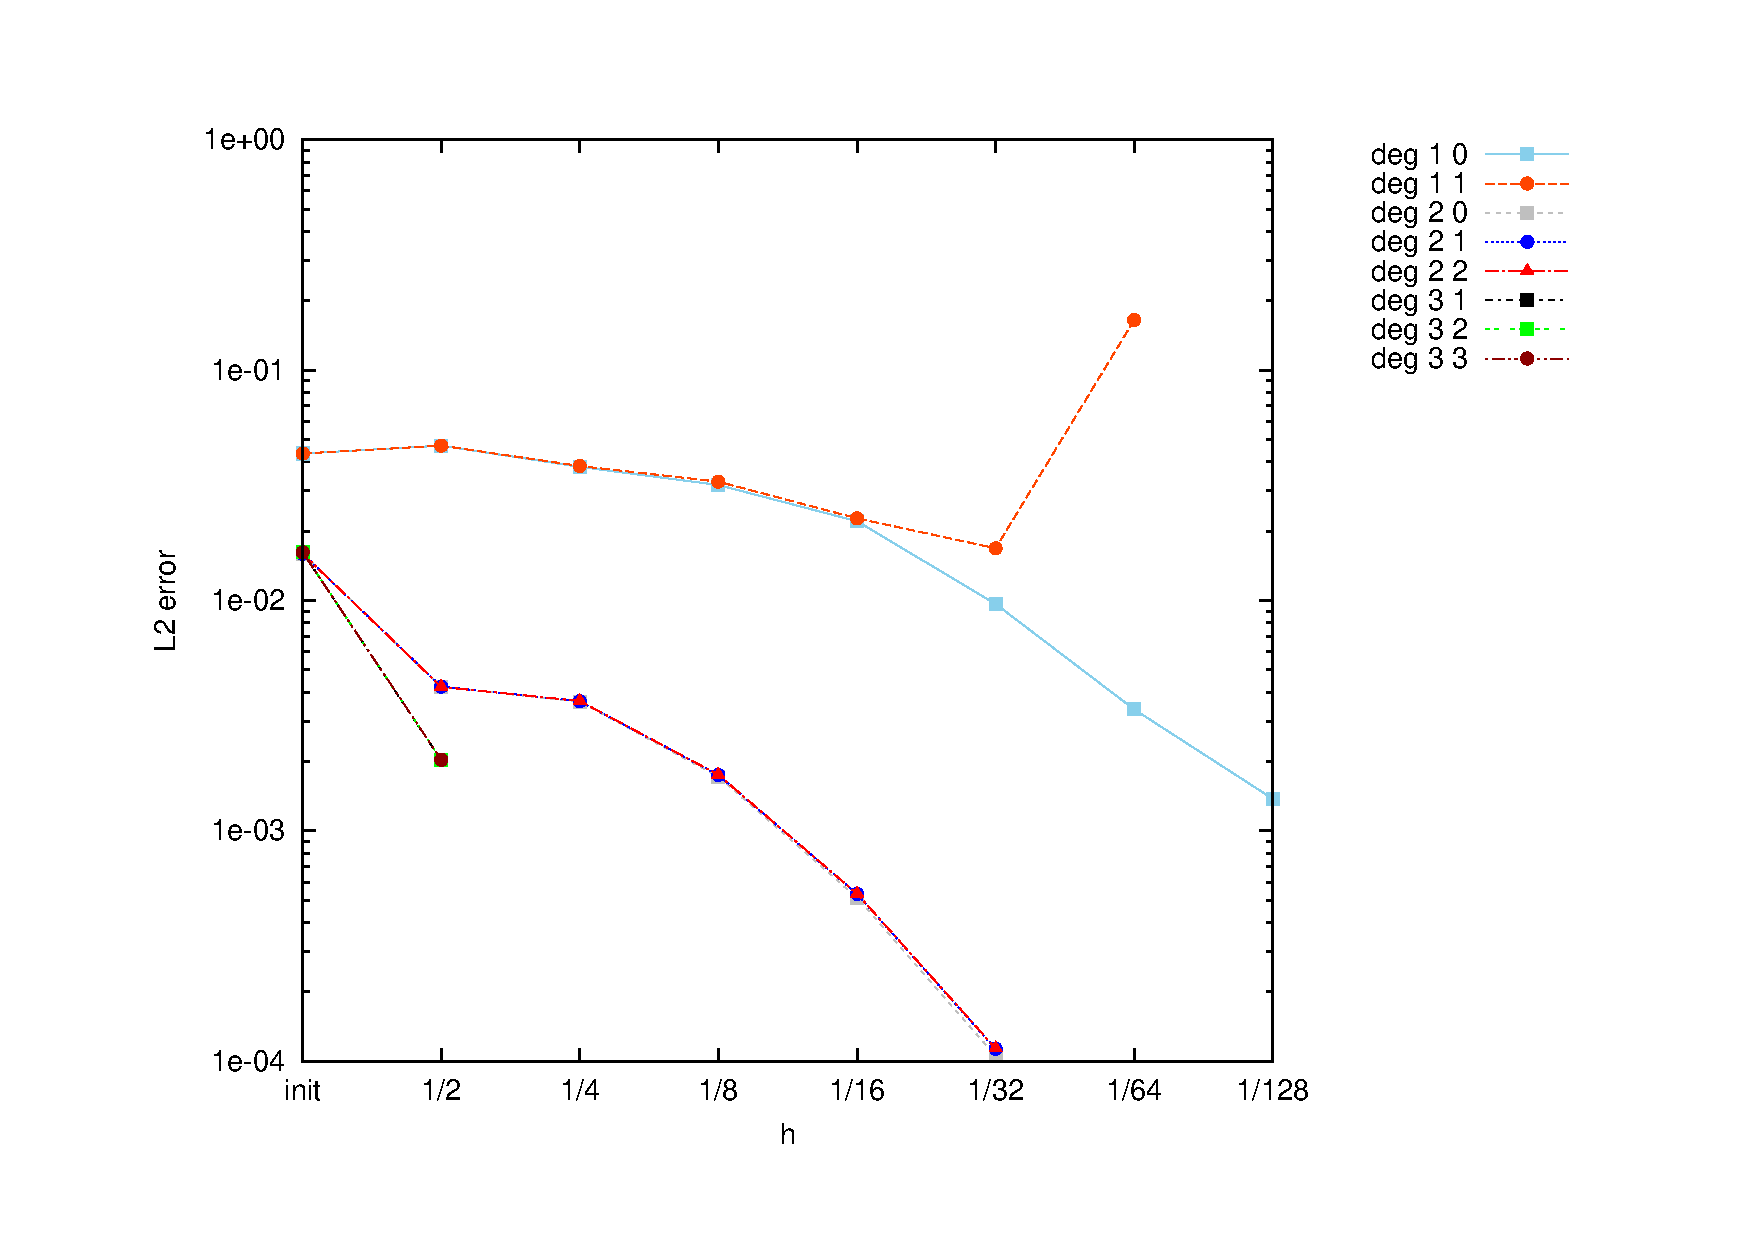
\includegraphics[scale =0.45]{plots/MA3_Neilan_GradJump_l2.pdf}
	\caption{$L^2$ errors for Test \ref{test singularity} and additional gradient jump penalty}
	\label{fig: l2 errors test 3 jump}
\end{figure}

\begin{figure}[H]
	\centering
	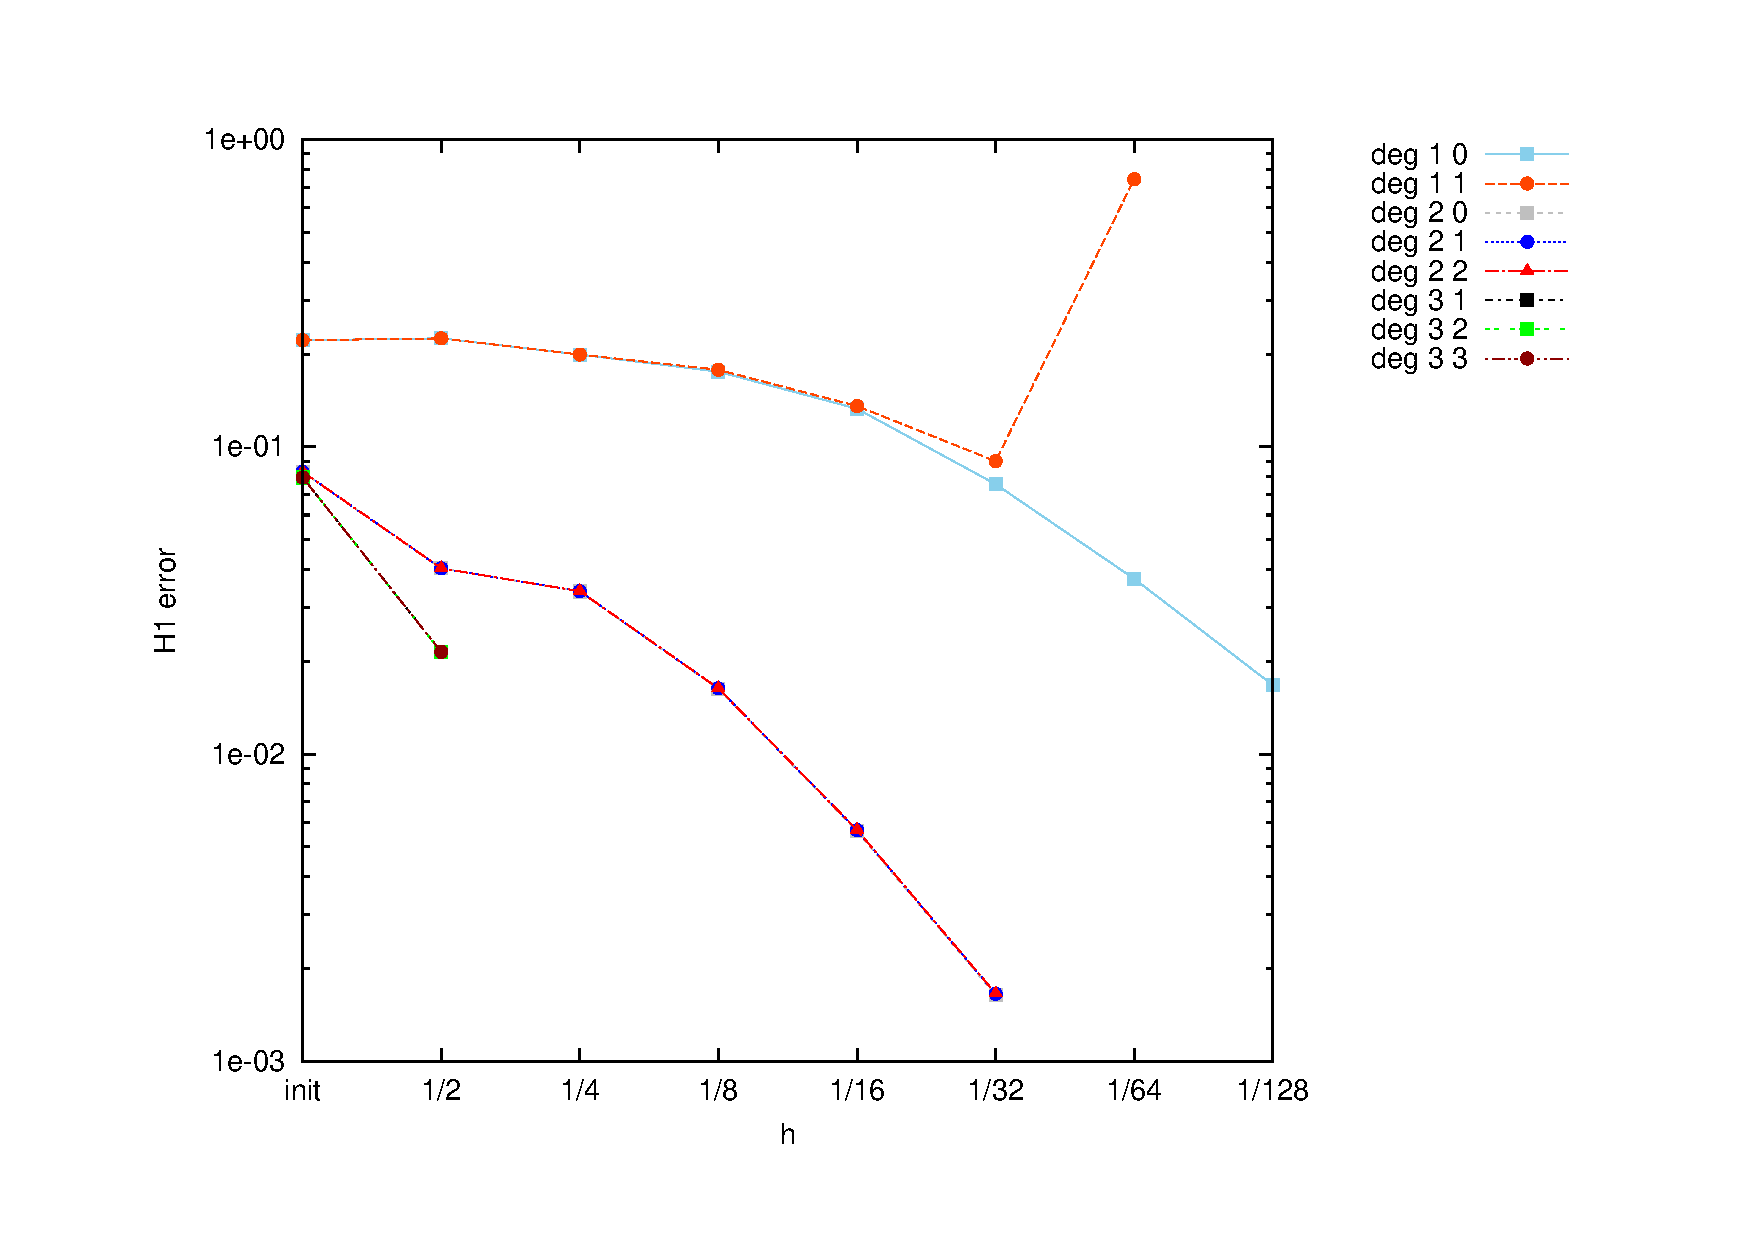
\includegraphics[scale =0.4]{plots/MA3_Neilan_GradJump_h1.pdf}
	\caption{$H^1$ errors for Test \ref{test singularity} and additional gradient jump penalty}
	\label{fig: h1 errors test 3 jump}
\end{figure}

\begin{table}[h]
	\begin{subtable}[b]{0.45\textwidth}
		\centering
		\pgfplotstabletypeset[columns={iterations, l2error, h1error,N},
		every row 0 column 0/.style={set content=init},
		]{\MAThreeJumpdegOneZero}
		\caption{Error for $k=1, k_{DH}=0$}
	\end{subtable}
	~
	\begin{subtable}[b]{0.45\textwidth}
		\centering
		\pgfplotstabletypeset[
		columns={iterations, l2error, h1error,N},
		every row 0 column 0/.style={set content=init},
		every row 6 column 1/.style={set content=-},
		every row 6 column 2/.style={set content=-},
		every row 6 column 3/.style={set content=-},
		every row 7 column 1/.style={set content=-},
		every row 7 column 2/.style={set content=-},
		every row 7 column 3/.style={set content=-},
		]{\MAThreeJumpdegTwoTwo}
		\caption{Error for $k=2, k_{DH}=2$}
	\end{subtable}
	\caption{Errors for Test \ref{test singularity} and additional gradient jump penalty}
	\label{tab: l2 errors test 3 jump}
\end{table}	

\begin{table}[H]
\centering
\begin{subtable}[b]{0.45\textwidth}
	\pgfplotstabletypeset
	{
		k $k_{DH}$ {numerical order}
		1 0 0.8565
		2 1 1.32222
		2 2 1.32048
	}
	\caption{numerical order in $L2$ norm}
	\end{subtable}
	\begin{subtable}[b]{0.45\textwidth}
	\pgfplotstabletypeset
	{
		k $k_{DH}$ {numerical order}
		1 0 0.618481
		2 1 1.17823
		2 2 1.17823
	}
	\caption{numerical order in $H1$ norm}
	\end{subtable}
	\caption{Numerical order with jump penalty in Test \ref{test singularity}}
\label{tab: order jump 3}
\end{table}




For the last test case the method without additional gradient jump were did not work out just as in the previous test cases. We therefore only concentrate on the performances penalising the normal gradient jump across edges. The error made is to be found in the plots in Figures \ref{fig: l2 errors test 3 jump} \ref{fig: h1 errors test 3 jump}, as wells as in Table \ref{tab: l2 errors test 4 jump}. Again Newton's method did not converge for $k=2,3$ on fine grids. 
\begin{table}[H]
	\begin{subtable}[b]{0.45\textwidth}
		\centering
		\pgfplotstabletypeset[columns={iterations, l2error, h1error,N},
		every row 0 column 0/.style={set content=init},
		]{\MAFourJumpdegOneZero}
		\caption{Error for $k=1, k_{DH}=0$}
	\end{subtable}
	~
	\begin{subtable}[b]{0.45\textwidth}
		\centering
		\pgfplotstabletypeset[
		columns={iterations, l2error, h1error,N},
		every row 0 column 0/.style={set content=init},
		every row 5 column 1/.style={set content=-},
		every row 5 column 2/.style={set content=-},
		every row 5 column 3/.style={set content=-},
		every row 6 column 1/.style={set content=-},
		every row 6 column 2/.style={set content=-},
		every row 6 column 3/.style={set content=-},
		every row 7 column 1/.style={set content=-},
		every row 7 column 2/.style={set content=-},
		every row 7 column 3/.style={set content=-},
		]{\MAFourJumpdegTwoTwo}
		\caption{Error for $k=2, k_{DH}=2$}
	\end{subtable}
	\caption{Errors for test case \ref{test dirac} and additional gradient jump penalty}
	\label{tab: l2 errors test 4 jump}
\end{table}


\begin{figure}[H]
	\centering
		\centering
		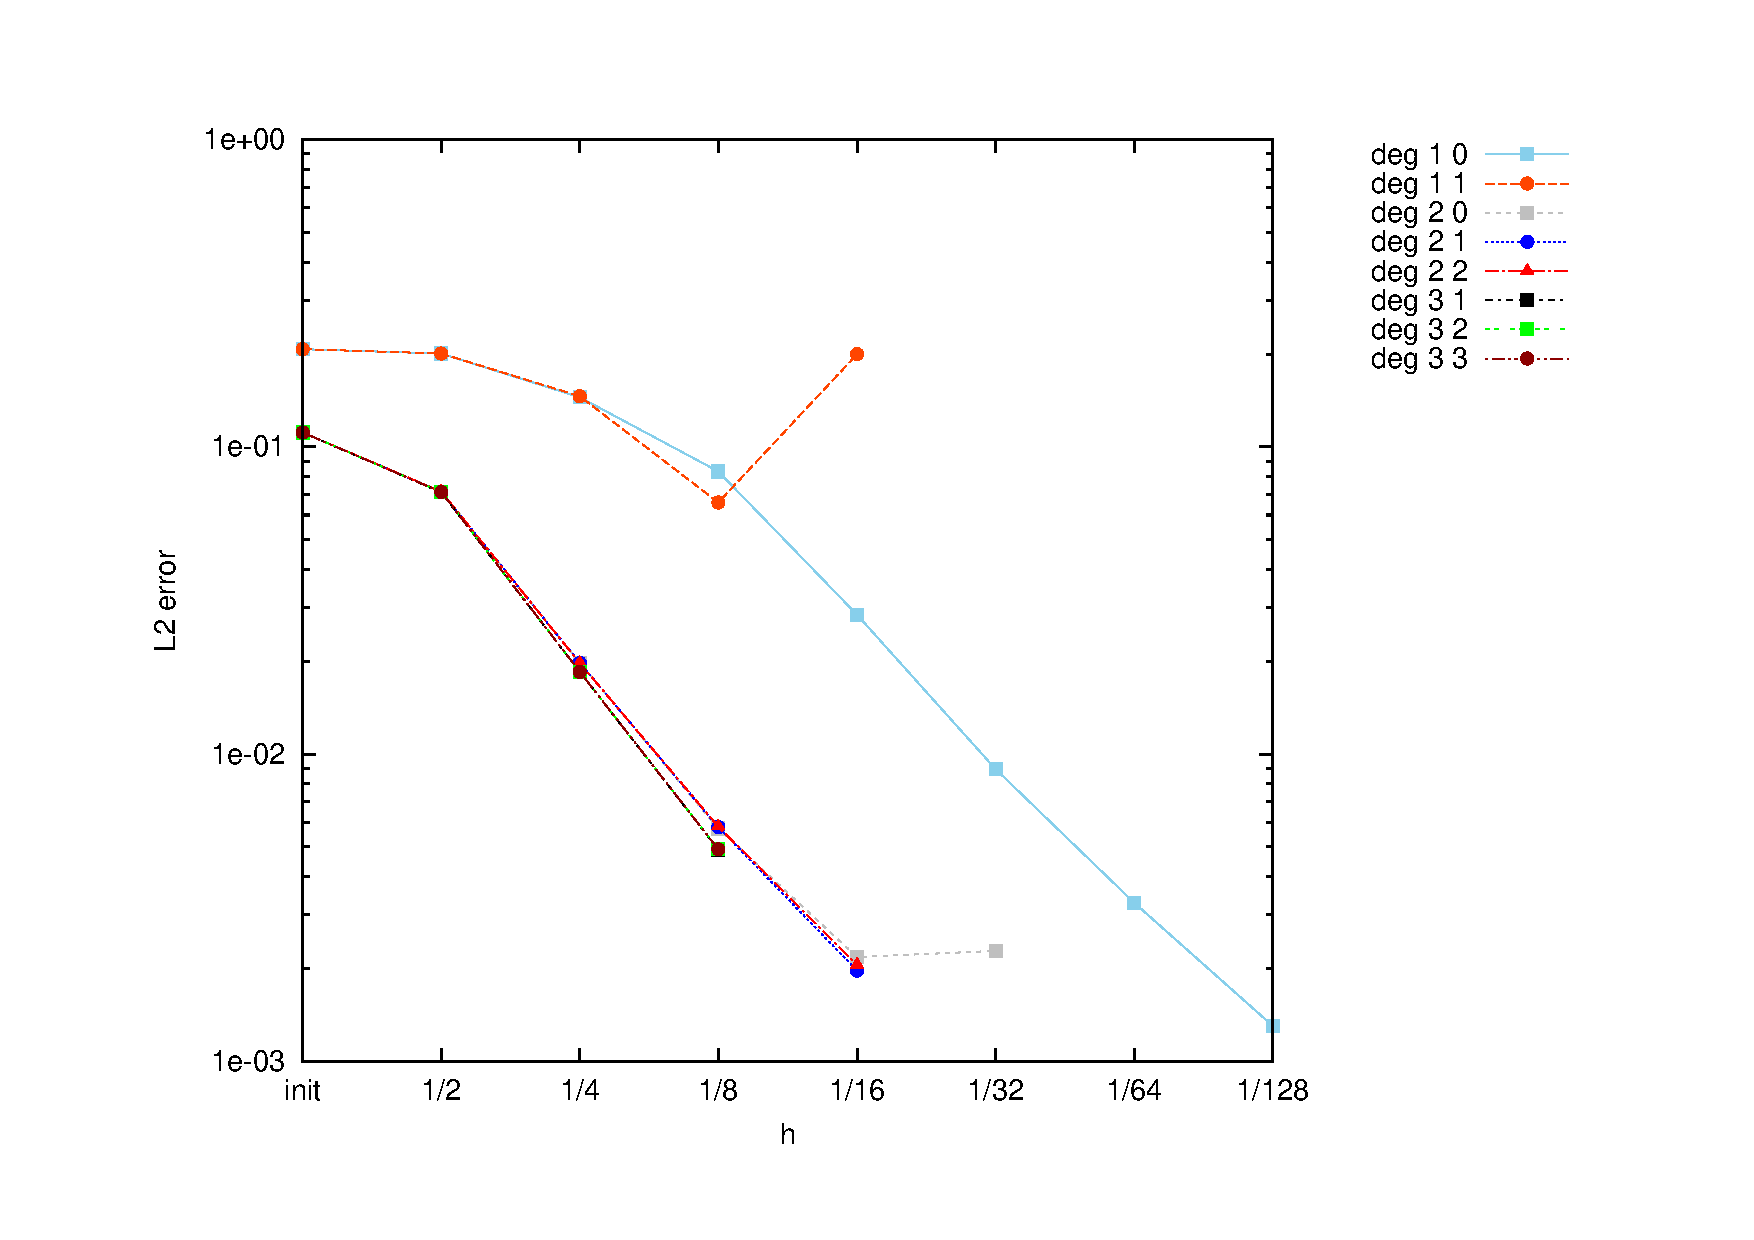
\includegraphics[scale =0.4]{plots/MA4_Neilan_GradJump_l2.pdf}
	\caption{$L^2$ errors for test case \ref{test dirac} and additional gradient jump penalty}
	\label{fig: l2 errors test 4 jump}
\end{figure}
	
\begin{figure}[H]
		\centering
		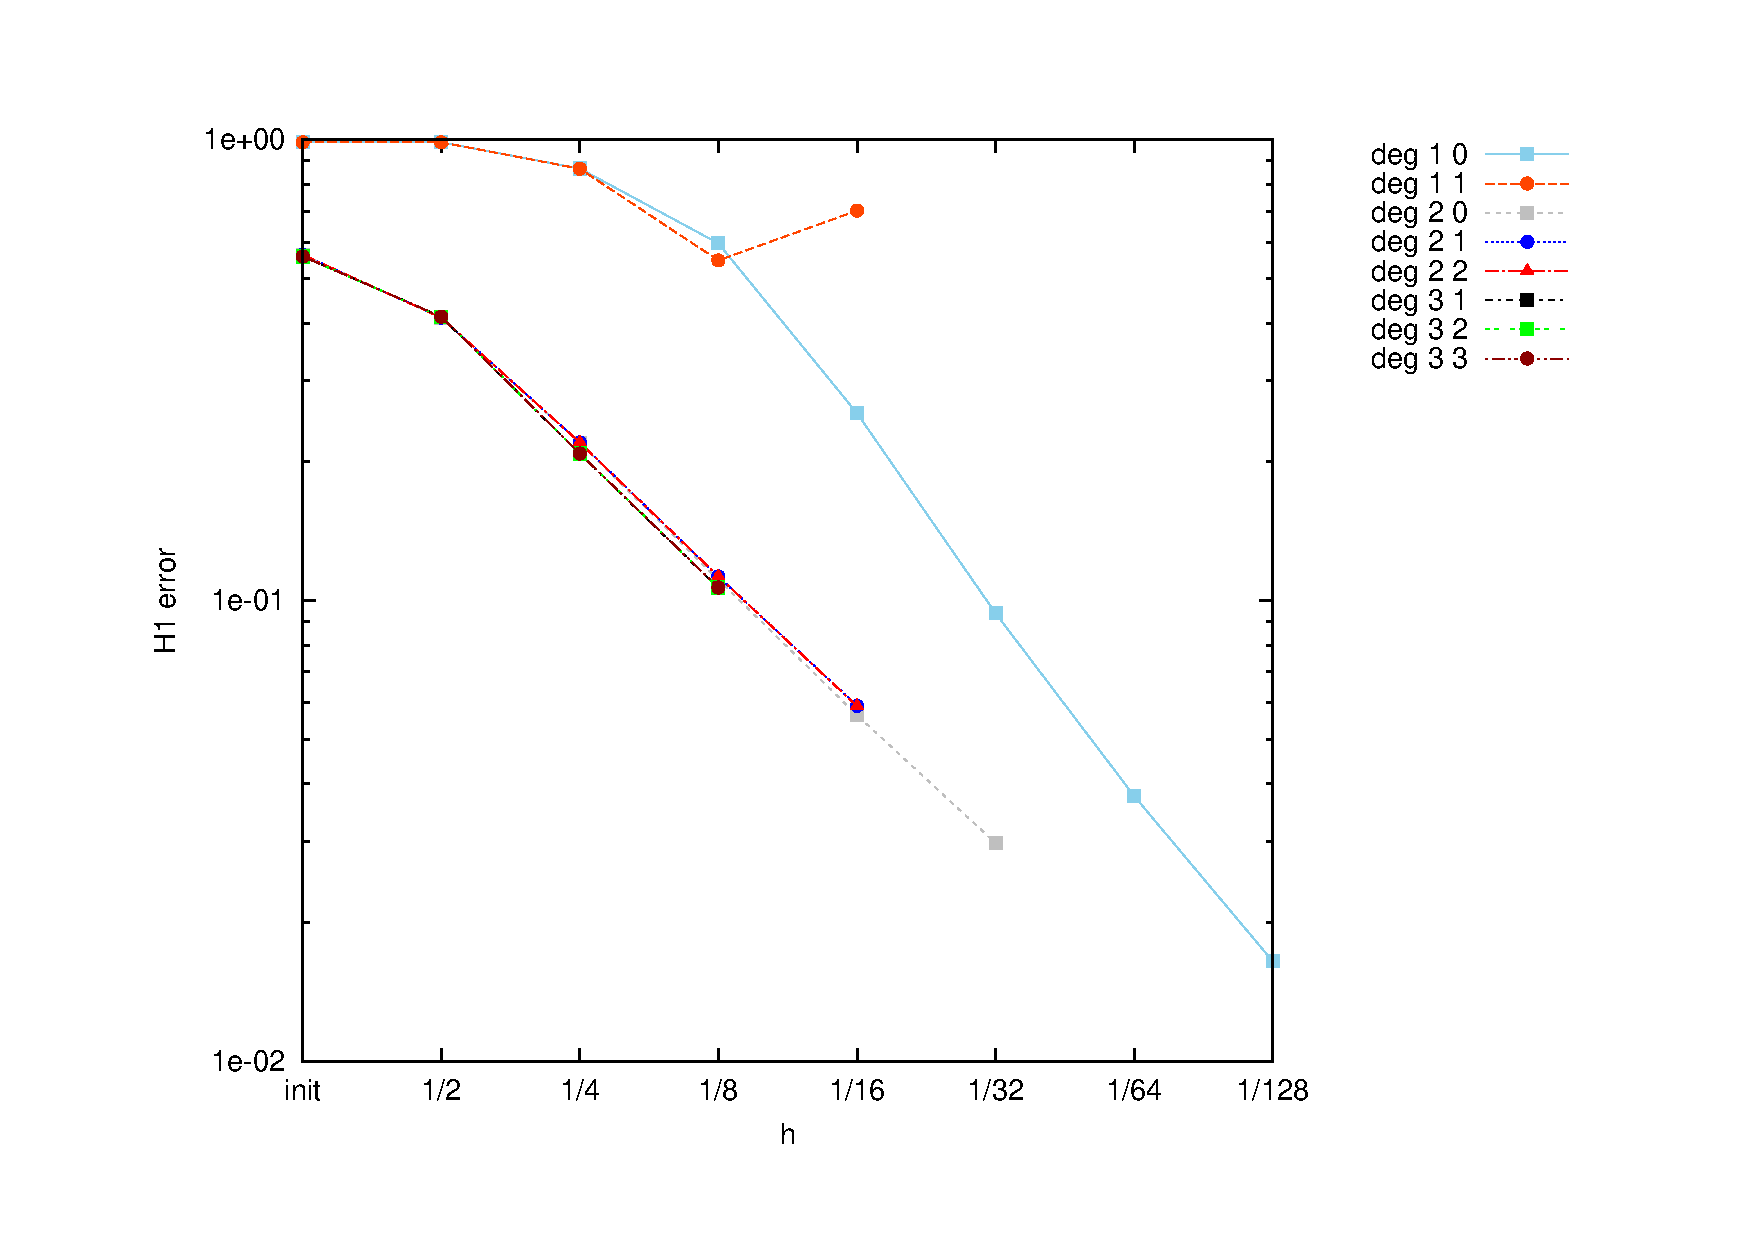
\includegraphics[scale =0.4]{plots/MA4_Neilan_GradJump_h1.pdf}
	\caption{$H^1$ errors for test case \ref{test dirac} and additional gradient jump penalty}
	\label{fig: h1 errors test 4 jump}
\end{figure}
As before we do not observe much difference between the choices $k=2$ and $k=3$ during the first (converged) refinements. But as the Aleksandrov solution of this test case lacks regularity it is not surprising that increasing the polynomial degree does not effect the error.

It is noticeable that for $k=2$ the $L^2$ error increases after four refinement while the $H^1$ error decreases, we already experienced this behaviour in test \ref{test smooth}.

\todo{symmetrised neilan and not crossed grid}

\newpage

\section{Numerical Results of DG Picard Iteration Method}

The Picard iteration is implemented in C++. All vector and matrix handling as well as was linear solvers are provided by the Eigen library \cite{eigenweb}. To solve the quadratic program arising in the context of a convexification (cf. \eqref{eq: convex lsq}) the C++ library ipopt \cite{ipopt} was used.

The C++ implementation uses the same nested grids as also have been used in the latter FEniCS implementations (cf. Figure \ref{fig: grids}). It is obtained by dividing the unitsquare along the diagonals into four triangles and then refining uniformly as explained in \ref{subsec: refinement and base cells}.

\subsection{Implementation Details}

The main class of the implementation is the Tsolver class. The solver collects all information and controls the assembly and solving process.
Hence, the main method which can be found in mesh.cpp just initialises solver and starts the solving process: Via a configuration file all input data is fed into the main routine. With this information the solver can initialise its members grid and Tshape, Those represent the underlying grid structure and the reference cell. 
The grid implemenation is taken from the igpm\_t2\_lib and is based on the work of \cite{BMV2009}.

The main method, i.e. the algorithm from Algorithm \ref{alg: final} is implemented in Tsolver's function stepping\_MA(). It starts with an initialisation process where it reads specific problem data which includes
\begin{enumerate}
 \item the problem we want to solve,
 \item penalty parameters to enforce continuity and penalise the gradient jump,
 \item the start level of refinement with respect to the initial grid $start\_level$,
 \item the damping paramter $\alpha$,
 \item the number of fixed point iterations per grid $max\_its$,
 \item the maximal grid refinements $max\_levelrefinement$.
\end{enumerate}
During the initialisation the methods also updates all base cell data and leaf cell data, enumerates the degree of freedoms and computes the initial guess.\\
Afterwards the fixed point iterations begins, in every step the General Poisson problem (cf. Section \ref{sec: SIPG MA}) solved, eventually convexified (cf. Section \ref{subsec: convexification}) and afterwards with the last solution step combined \ref{subsec: add penalty param}). If the specified number of iterations has been carried out, the grid is refined, the leaf cell data updated and we start the fixed point iterations again.
We repeat this process until the maximal number of grid refinements is reached.
To illustrate this procedure Algorithm \ref{alg: stepping} shows the function stepping\_MA() in pseudo code.
\begin{algorithm}[H]
\begin{algorithmic}
	\State Read problem specific data
%		\begin{enumerate}
%			 \item  problem\_name \Comment {to choose right-hand side and boundary conditions}
%			 \item penalty parameters   \Comment {  to enforce continuity and penalise the gradient jump}
%			 \item start\_level  \Comment { the start level of refinement with respect to the input grid}
%			 \item $\alpha$  \Comment {the damping paramter}
%			 \item maxits \Comment{ the number of fixed point iterations per grid}
%			 \item max\_levelrefinement \Comment{ the maximal refinement level }
%		\end{enumerate}
	\State Initialise base cell data
	\State Refine to $start\_level$
	\State Initialise leaf cell data
	\State Enumerate degree of freedoms
	\State (Initialise Convexifier)
	\State Initialise initial guess $u_{-1}$
	\State level $\gets start\_level$
	\State $i \gets 0$
	\While {level < $max\_levelrefinement$}
		\State Enumerate degree of freedoms
		\State Update base and leaf cell data
		\State (Initialise C0 converter) \Comment{only needed for convexification}
		\State cur\_it$ \gets 0$
		\While {cur\_it < $maxits$}
			\State  assemble\_MA()                              \Comment Assemble system for General Poisson problem
			\State $u_i \gets$ solution of assembled system
			\State (Convexify $u_i$)		 
			\State $u_i \gets \alpha u_{i-1}  +(1-\alpha) u_i$
			\State	cur\_it, i $\gets$ cur\_it$+1$, i$+1$
			\State Restore\_MA() 		\Comment{Store solution in leaf cells}
		\EndWhile
		\State Refine grid and update leaf cell data
		\State level $\gets$ level $+1$
	\EndWhile
\end{algorithmic}
\caption{stepping\_MA}
\label{alg: stepping}
\end{algorithm}

After we have seen the program structure I shortly remark some of arising programming issues:

Before the actual system assembly the diffusion matrix in every cell has to be updated with the modified cofactor matrix of the Hessian of the last Picard step. Note that this matrix is constant for polynomial degree $k=2$ and otherwise has to be calculated at every quadrature point. Since in general here is no connection between diffusion matrix values at the reference cell and in the leaf cell, we cannot save easily any memory as we did for function values and normal gradients (cf. Section \ref{subsec: ref cell} and \ref{subsec: refinement and base cells}). Hence, we store the diffusion matrix at every quadrature point on the grid in the corresponding leaf cell.
The rest of the assembly process is carried out as already mentioned in algorithm \ref{alg: assembling}. Hereby one has to pay attention to the right scaling of quadrature weights and the right calculation of quadrature data from reference cell data as described in Examples \ref{ex: base cell trafo} and \ref{ex: leaf cell trafo}. 

If a convexification is desired, the class Convexifier takes care of the execution of the method described in Section \ref{subsec: convexification}. The linear constraints ensuring convexity on a triangle are chosen the one from theorem \ref{thm: convex cond on triangle} and the constrains for convexity across edges were given by theorem \ref{thm: convex cond across edge}. Due to the error-proneness during the assembly of $C$ the convexification was only implement for the case $k=2$. Note that before applying the theorems we have to convert our numerical solution from the DG formulation to a $C^0$ spline.
Hence, the Convexifier computes at first using the C0converter the $C^0$ spline representation of the Poisson solution and then assembles the matrices $A$ and $C$ of \eqref{eq: convex lsq}. To solve the problem it makes use of the open source library ipopt \cite{ipopt}.\\
Fortunately the evaluation matrix $A$, and the constraint matrix $C$ of \eqref{eq: convex lsq} only depend on the grid and thus, need only to be assembled once in every refinement.

Additionally the Tsolver has a member Plotter handling all export to external files. It is able to write the solution which's coefficients are currently stored in the leaf cells to a .vtu file or .dat file. Besides plotting it also administers all file streams to which information such as $L^2$ errors are written into.

\subsection{Results with Convexification}

For a initial guess I also used the solution of $\triangle u = -\sqrt{2f}$ combined with the multilevel approach as described in \ref{sec: initial guess}.
The arising linear system of equations was solved with Eigen's internal Cholesky solver.
The parameters were if not other specified taken to be $\sigma=10 k^2, \sigma_G = 50, \alpha =
0.3$ and $\varepsilon = 1e-2$. We always carry out 15 steps including a convexification after every step before we refine further. The implemented convexification followed the ideas of Section \ref{subsec: convexification}. 


The results shown in figure \ref{fig: l2 errors test smooth ourMethodConvex} show the method does not work as expected.
\begin{figure}[H]
\centering
	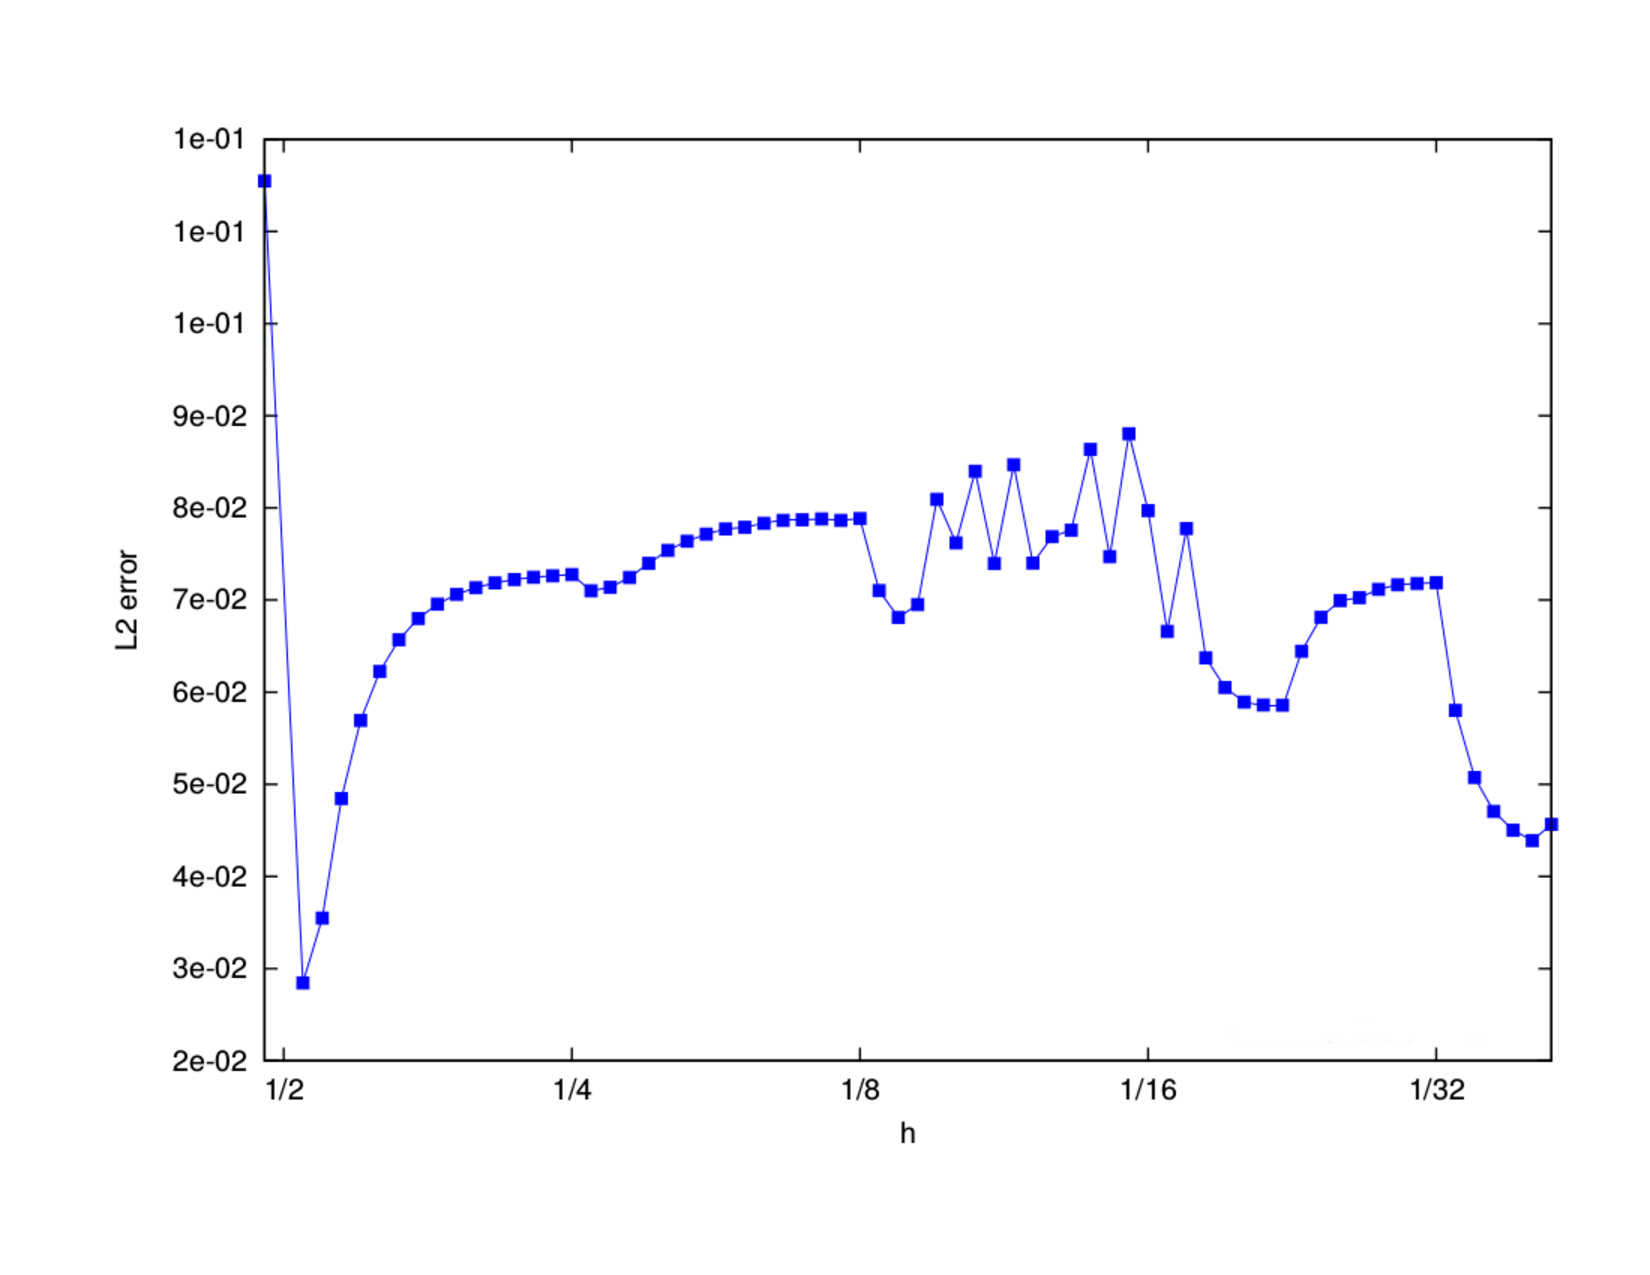
\includegraphics[scale =0.4]{plots/MA1_convexify.pdf}
	\caption{$L^2$ errors for test case \ref{test smooth} and additional convexification}
	\label{fig: l2 errors test smooth ourMethodConvex}
\end{figure}
To investigate the cause of this failure we give in Figure \ref{fig: convex before after} the plot of the $L^2$ error before the convexification step and the plot after it. As we can see the convexification process increases the error. There are several possible explanations for that:

Though the convexification algorithm produces a convex result it does not garantuee that it leaves convex input functions unchanged.

The convex function in $\mathcal P^2_h$ approximating the numerical solution $u_h$ best is not necessarily closer to the exact solution $u$ than $u_h$. Then the convexification gives a push into the wrong direction.

The best approximation of $u$ into $\mathcal P^2_h$ does not have to be convex, for example the affine Lagrange interpolant of a convex function does not to be convex\cite[p.3142]{AM2009}. 

To understand how \quoting{unconvex} the function was before the convexification process I have examined the vector $Cc_u$ where $C$ is the matrix containing the convexity conditions and $c_u$ are the coefficients of $L2$ projection into $\mathcal P^2_h$: The minimal entry for a grid with $h=1/2$ is -9.77e-03, for a grid with $h=1/16$ the minimal entry is -4.26e-04. Thus, the $L2$ projection of the exact solution does not comply with the convexity conditions.
Figure \ref{fig: convex min coeffs} plots the minimal entry of $Cc$ during the Picard iterations. We see that especially for small grid widths the Poisson solutions do not fulfill the convexity conditions. 

\begin{figure}[H]
\centering
	\begin{subfigure}{0.45\textwidth}
		\centering
		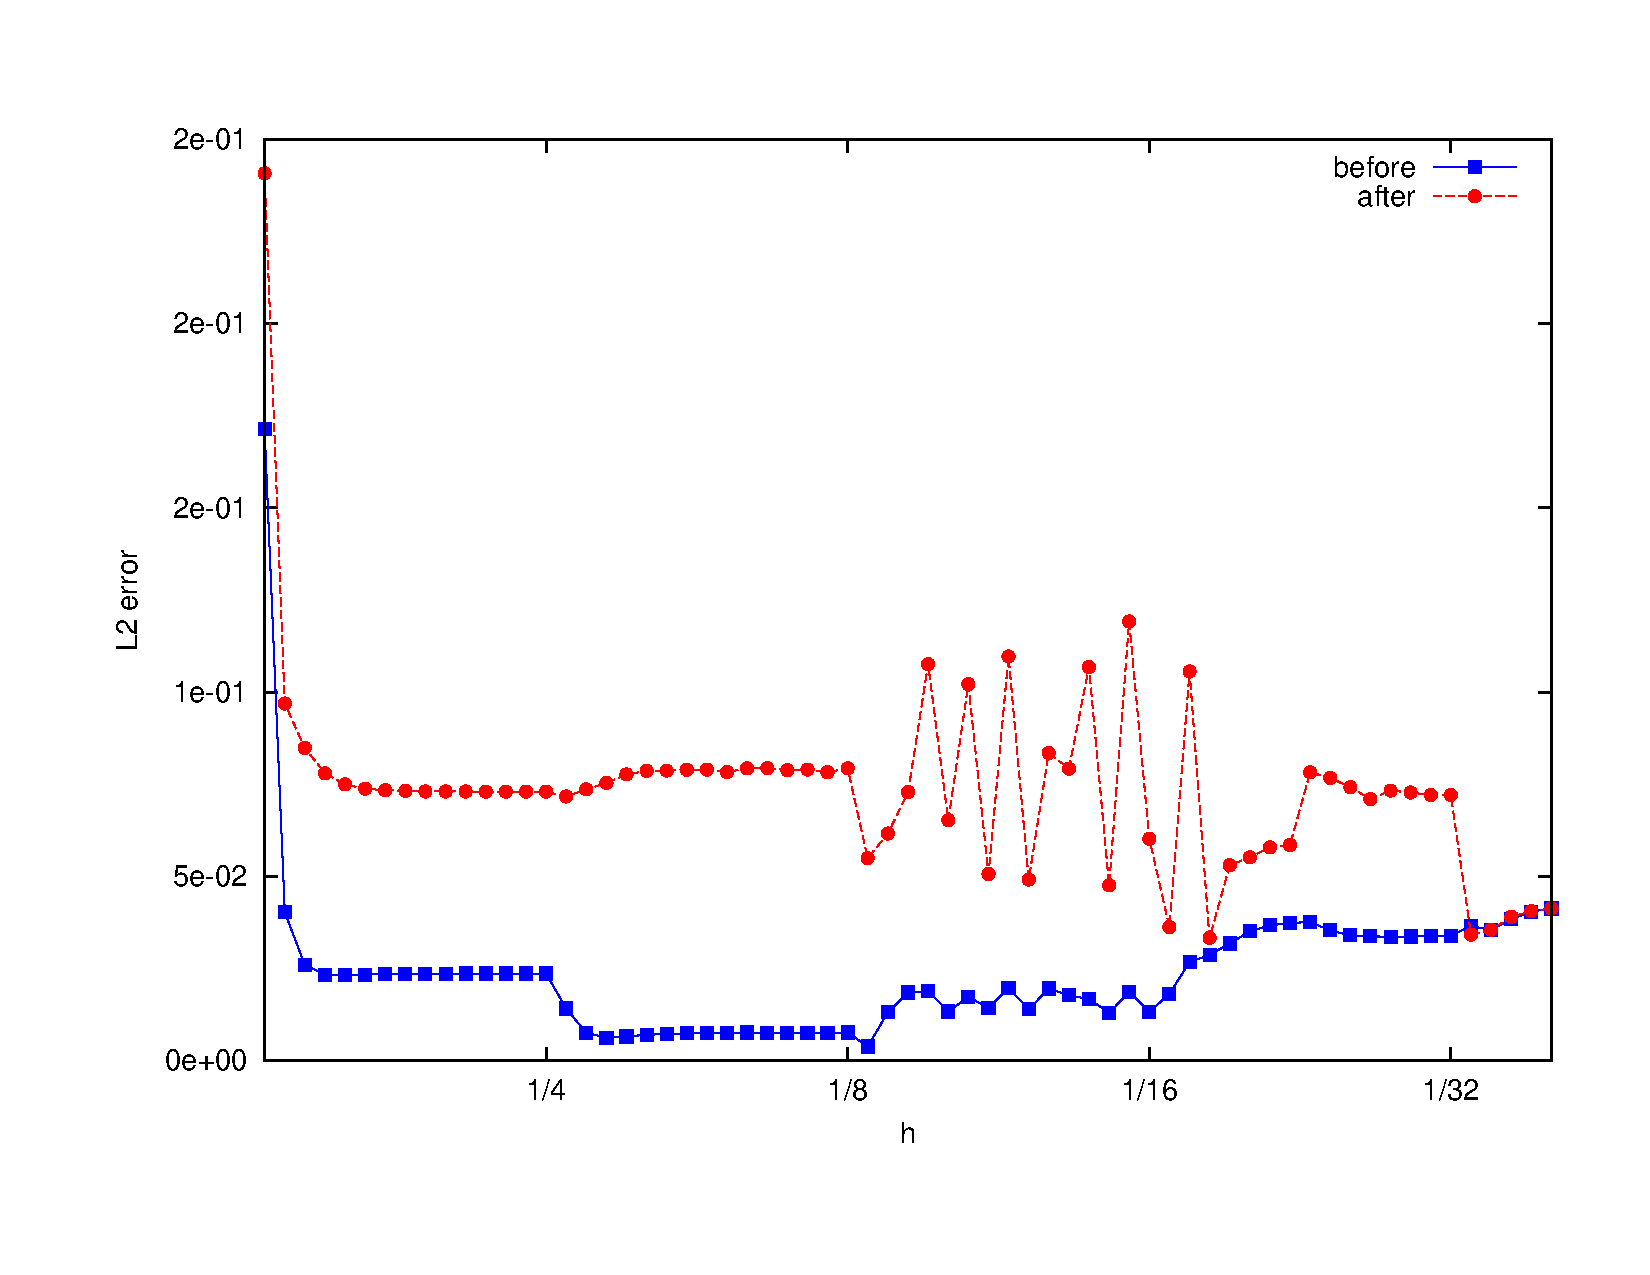
\includegraphics[scale=0.25]{plots/MA1_convexComp.pdf}
		\caption{Comparison of $L^2$ errors directly before and after convexification}
		\label{fig: convex before after}
	\end{subfigure}
	\begin{subfigure}{0.45\textwidth}
		\centering
		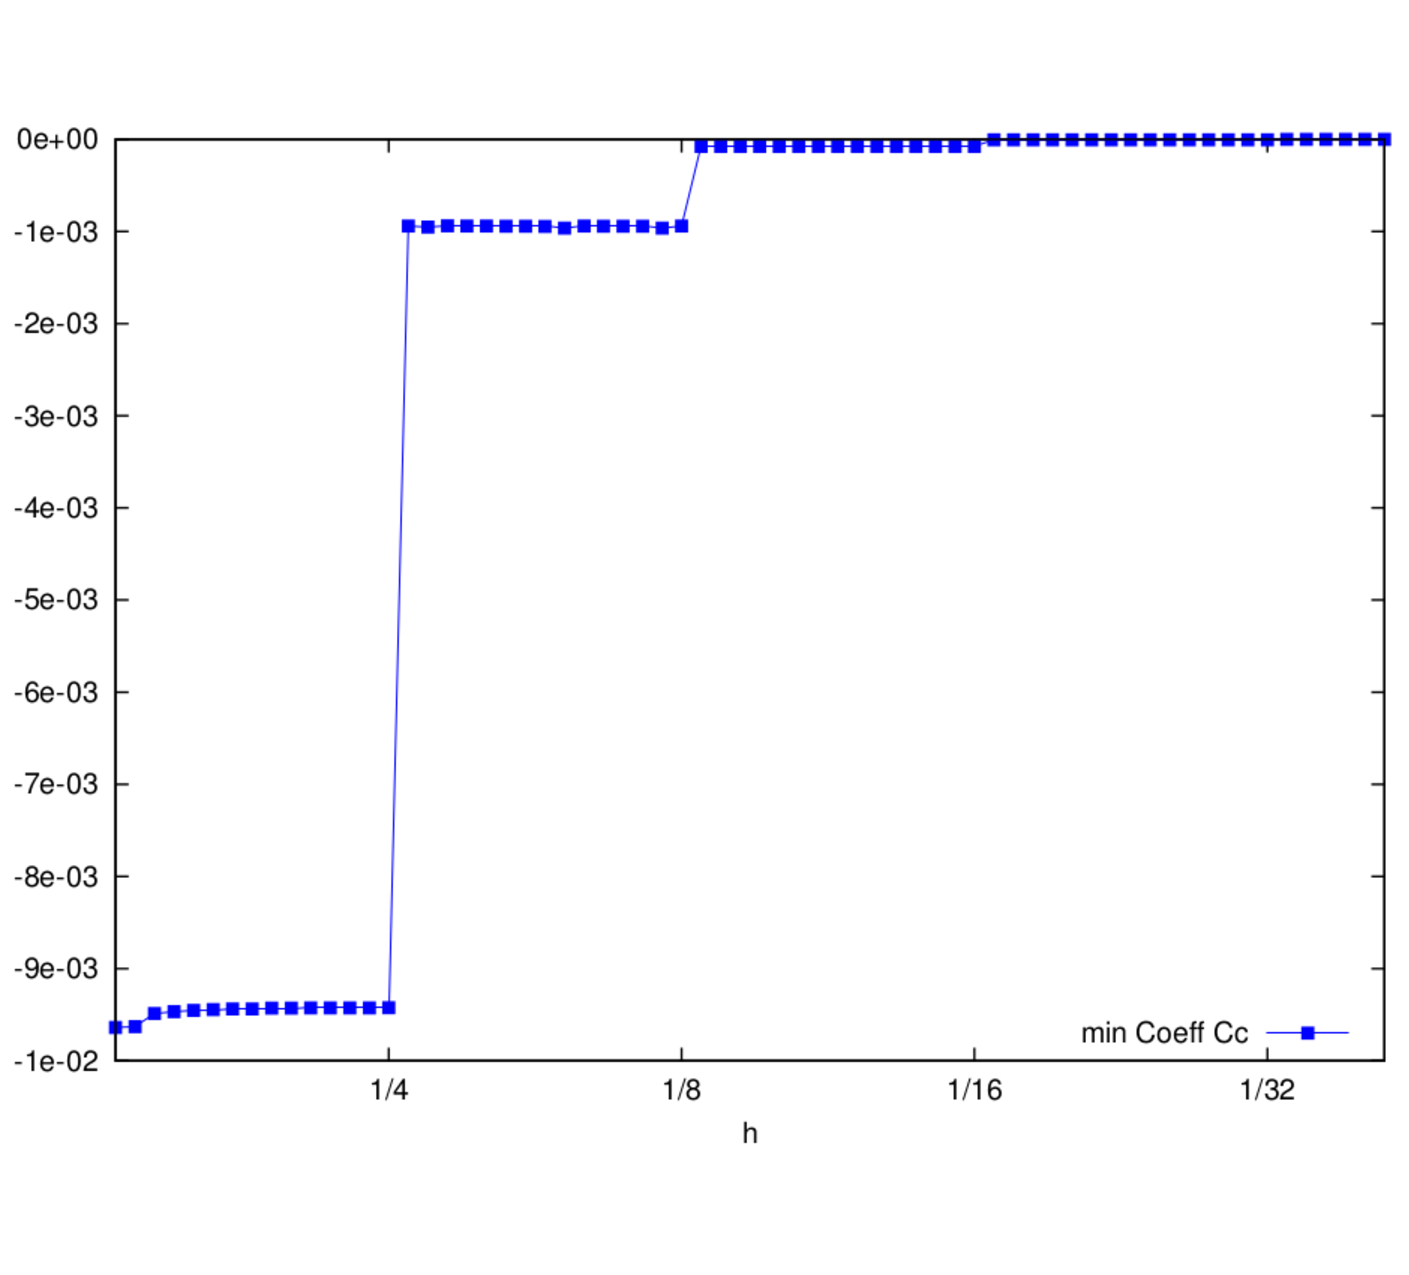
\includegraphics[scale=0.25]{plots/MA1_minCoeff.pdf}
		\caption{Comparison of $L^2$ errors directly before and after convexification}
		\label{fig: convex min coeffs}
	\end{subfigure}	
	\caption{$L^2$ errors for test case \ref{test smooth} and additional convexification}
	\label{fig: Compare test smooth ourMethodConvex}
\end{figure}


The other test cases produce similar results such that we can assume the presented convexification is not sensible in the context of the Picard iteration.

%\begin{figure}[H]
%\centering
%	\includegraphics[scale =0.4]{plots/MA2_convexify.pdf}
%	\caption{$L^2$ errors for test case \ref{test singularity} and additional convexification}
%	\label{fig: l2 errors test singularity ourMethodConvex}
%\end{figure}
%\begin{figure}[H]
%\centering
%	\includegraphics[scale =0.4]{plots/MA2_convexComp.pdf}
%	\caption{$L^2$ errors for test case \ref{test singularity} and additional convexification}
%	\label{fig: Compare test singularity ourMethodConvex}
%\end{figure}


	

\subsection{Results without Convexification}

We used the same code basis as in the previous tests but turned off every direct convexification.
In Figure \ref{fig: l2 errors test smooth ourMethod} and Table \ref{tab: l2 errors our method} can see the results for the the smooth test case \ref{test smooth}.
\begin{figure}[H]
	\centering
	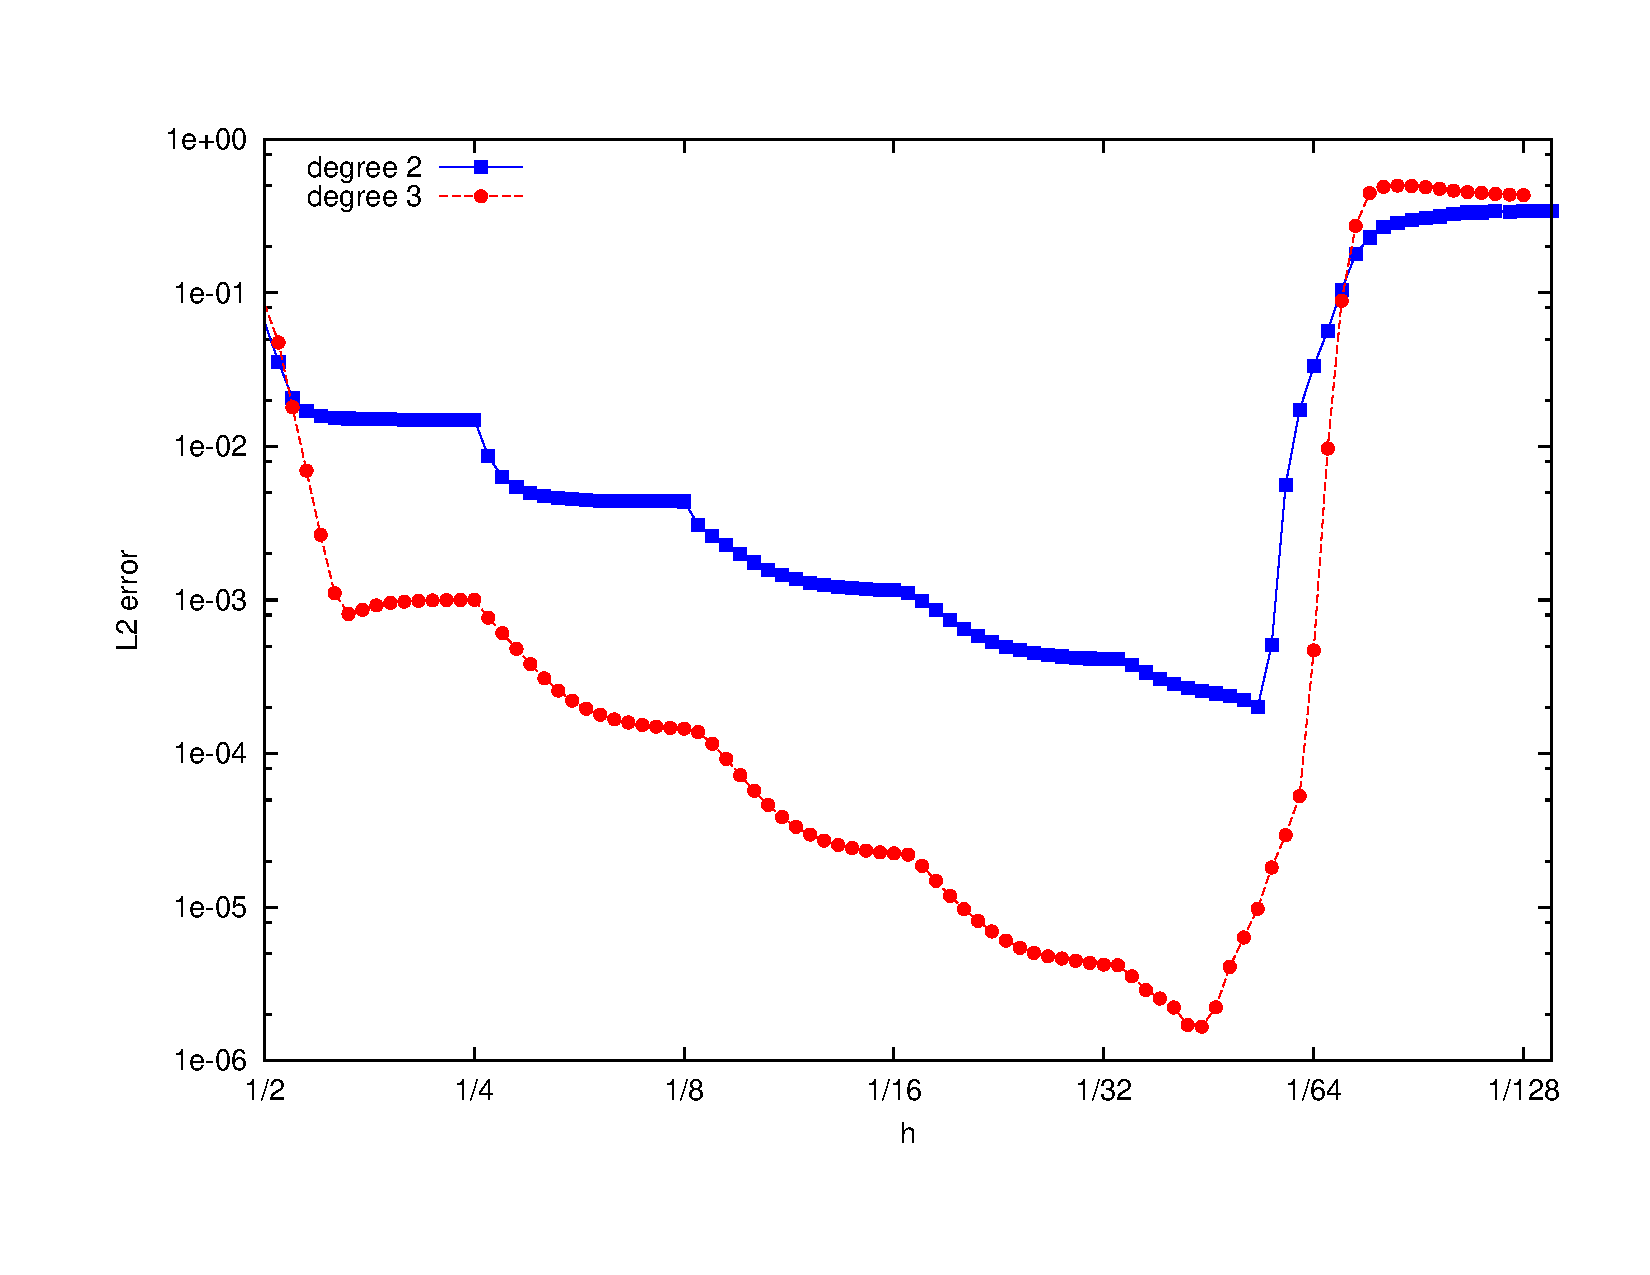
\includegraphics[scale =0.4]{plots/MA1.pdf}
	\caption{$L^2$ errors for test case \ref{test smooth}}
	\label{fig: l2 errors test smooth ourMethod}
\end{figure}
\begin{table}[H]
	\centering
	\begin{subtable}[b]{0.45\textwidth}
		\centering
		\pgfplotstabletypeset[
			every first column/.style={string type},
		    every second column/.style={
		    dec sep align,      % align on the decimal marker
		    /pgf/number format/sci e, 
		    /pgf/number format/fixed zerofill=true,  % print trailing zeros
		    /pgf/number format/sci precision=4     % print 14 digits
			}
		]
		{
		{$h$}  l2error
		{init}  0.117041 
		{$1/2$}  0.0247946 
		{$1/4$}  0.0094535 
		{$1/8$}  0.00181535 
		{$1/{16}$}  0.000435754 
		{$1/{32}$}  0.00015778 
		{$1/{64}$}  0.248114				
		}
		\caption{$L^2$ error for $k=2$}
	\end{subtable}
	\begin{subtable}[b]{0.45\textwidth}
		\centering
		\pgfplotstabletypeset[
		every first column/.style={string type},
		every second column/.style={
			dec sep align,      % align on the decimal marker
			/pgf/number format/sci e, 
			/pgf/number format/fixed zerofill=true,  % print trailing zeros
			/pgf/number format/sci precision=4     % print 14 digits
		}
		]
		{
			{$h$}  l2error
			{init}  0.151794
			{$1/2$} 0.00101133
			{$1/4$}  0.000140753
			{$1/8$}  2.10612e-05
			{$1/{16}$}  3.9589e-06
			{$1/{32}$}  3.46521e-06
			{$1/{64}$}  0.557331				
		}
		\caption{$L^2$ error for $k=3$}
	\end{subtable}
	\caption{$L^2$ errors for test \ref{test smooth}}
	\label{tab: l2 errors our method}
\end{table}


 For the first four refinements the method behaves well for both $k=2$ and $k=3$. Afterwards the numerical solution departs from the actual solution.
 
 We get similiar results in the next two cases albeit the fixed point iterations performs worse in the second case which lacks $H^2$ regularity. The $L2$ errors are shown in the Figures \ref{fig: l2 errors test sqrt ourMethod} and \ref{fig: l2 errors test singularity ourMethod}.
 
\begin{figure}[H]
\centering
	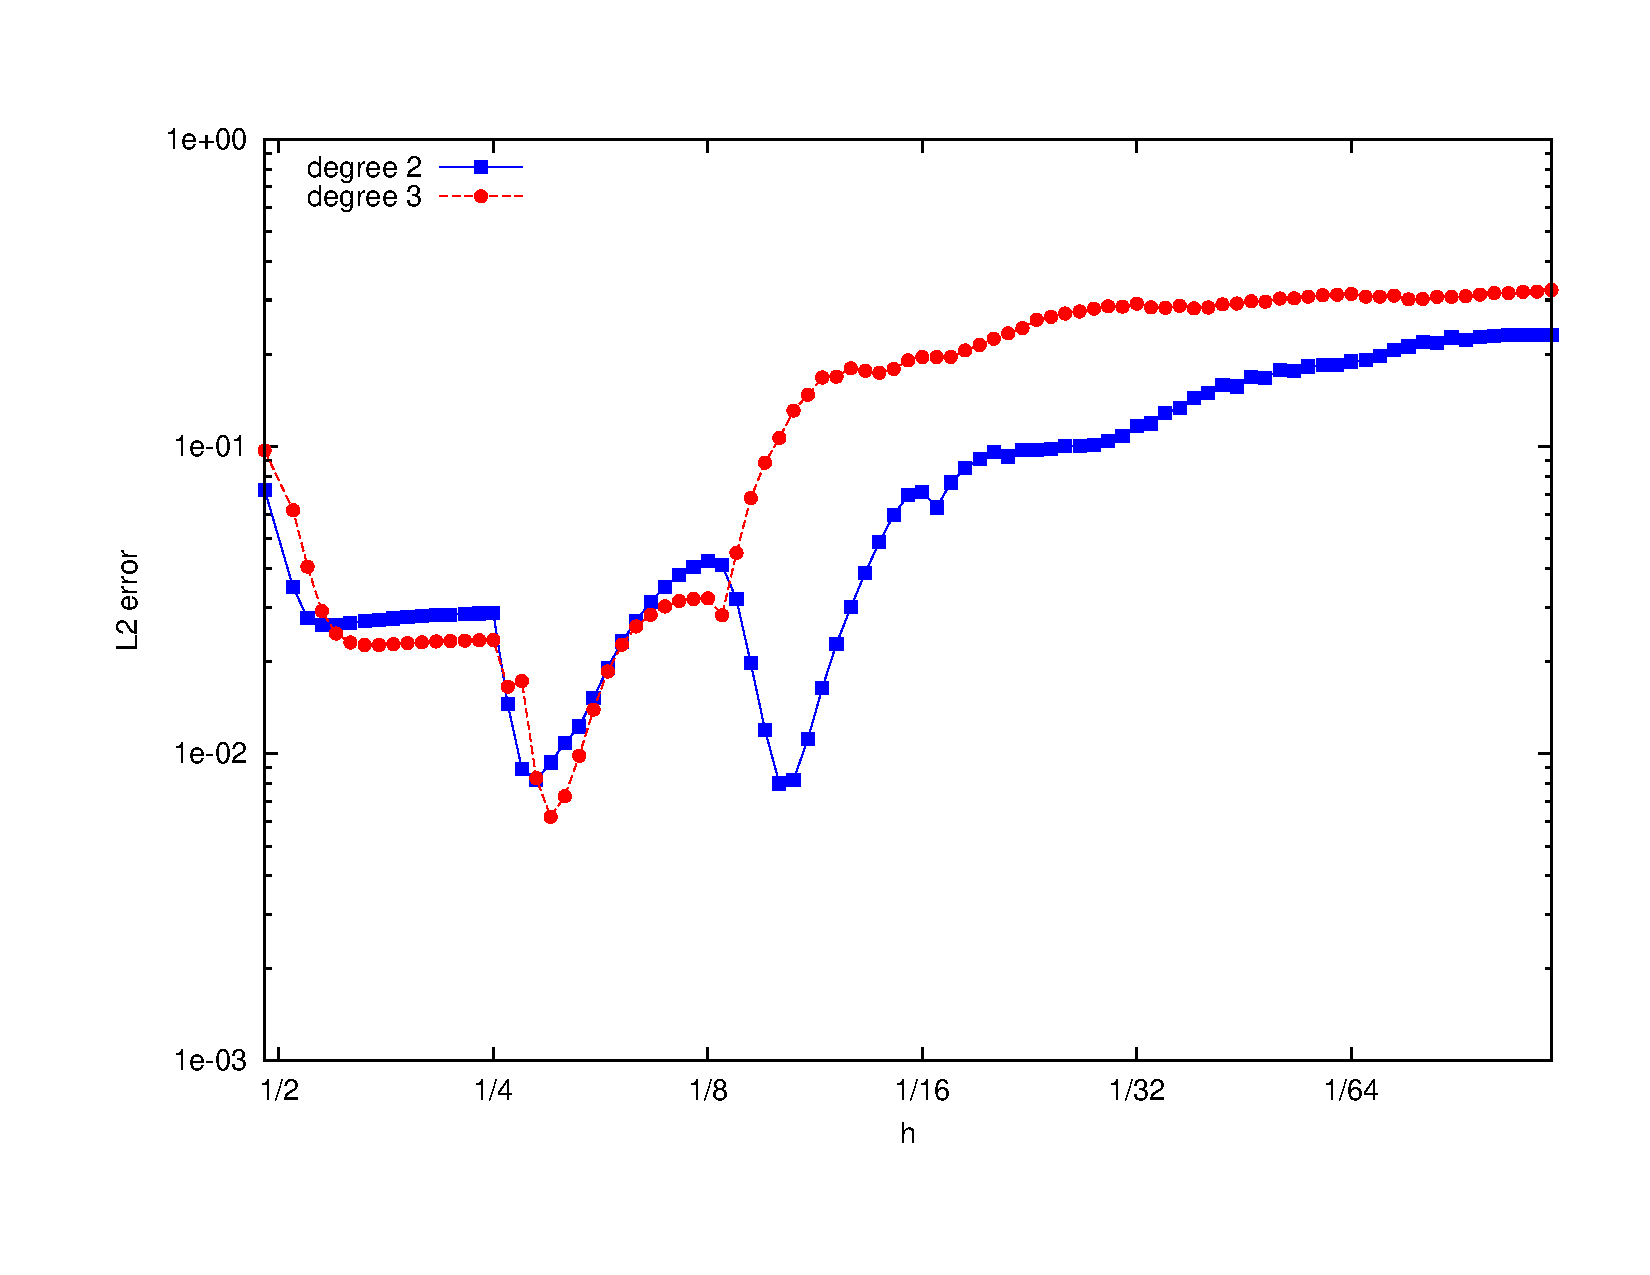
\includegraphics[scale =0.4]{plots/MA3.pdf}
	\caption{$L^2$ errors for test case \ref{test sqrt}}
	\label{fig: l2 errors test sqrt ourMethod}
\end{figure}


\begin{figure}[H]
\centering
	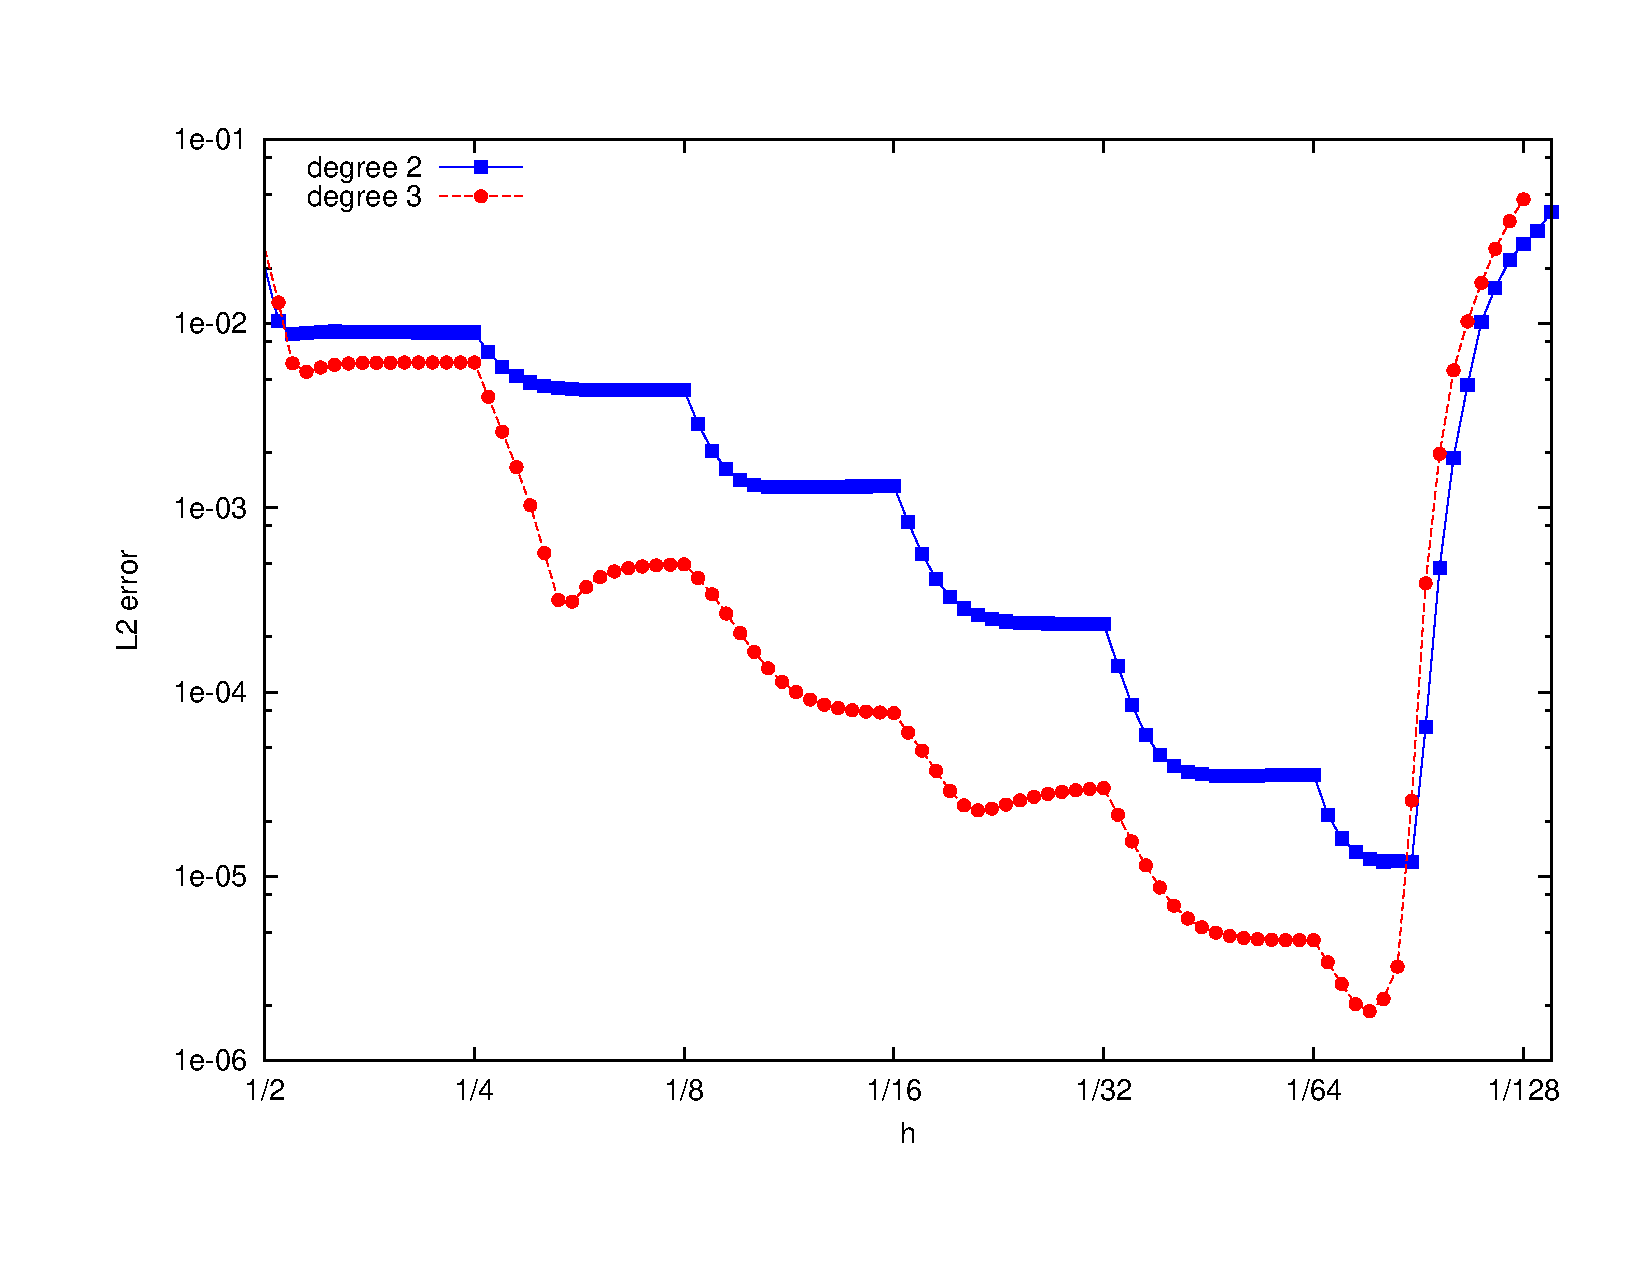
\includegraphics[scale =0.4]{plots/MA2.pdf}
	\caption{$L^2$ errors for test case \ref{test singularity}}
	\label{fig: l2 errors test singularity ourMethod}
\end{figure}

The results were validated by a reference implementation using the finite element tool FEniCS. Albeit I was not able to include the modified cofactor matrix to the bilinear form the error behaved as in the computational results of the C++ code. It decreased for the first four refinements and diverged afterwards. 

Additionally one can in the FEniCS variant the cofactor matrix of the Hessian which is evaluated piecewise replace by the discrete Hessian as defined in \ref{def: discrete Hessian} for a symmetric ansatz space $\Sigma_h$. The code can be found in the Appendix \todo{ref}.